\documentclass[12pt,a4paper,oneside]{report}

% ---------------------------------------------------------------- layout (EC418 BISP report format: A4, Times,
% 12 pt, 1.5 line spacing, justified, page number at the bottom centre)
\usepackage[a4paper,left=38mm,right=25mm,top=25mm,bottom=25mm,footskip=12mm]{geometry}
\usepackage[T1]{fontenc}
\usepackage[utf8]{inputenc}
\usepackage{mathptmx}
\renewcommand{\ttdefault}{pcr}
\usepackage{setspace}
\setstretch{1.45}
\usepackage{graphicx}
\usepackage{tabularx}
\usepackage{xltabular}
\usepackage{array}
\usepackage{enumitem}
\usepackage{amsmath}
\usepackage[labelfont=bf,labelsep=colon,font=small,justification=centering,singlelinecheck=true]{caption}
\captionsetup[table]{position=top,skip=4pt}
\captionsetup[figure]{skip=6pt}
\usepackage{float}
\usepackage{tikz}
\usetikzlibrary{positioning,fit}
\usepackage{cite}
\usepackage{titlesec}
\usepackage{titletoc}
\usepackage{url}
\usepackage[hidelinks]{hyperref}
\urlstyle{same}
\setlength{\parskip}{6pt}
\setlength{\parindent}{0pt}
\renewcommand{\arraystretch}{1.25}
\usepackage{etoolbox}
\AtBeginEnvironment{table}{\setstretch{1.05}}
\AtBeginEnvironment{xltabular}{\setstretch{1.05}}
\AtBeginEnvironment{longtable}{\setstretch{1.05}}
\newcolumntype{L}{>{\raggedright\arraybackslash}X}
\newcolumntype{P}[1]{>{\raggedright\arraybackslash}p{#1}}
\setlist{itemsep=2pt,topsep=4pt}
\setlist[itemize]{label=\textbullet,leftmargin=12mm}
\setlist[enumerate]{leftmargin=12mm}

% page number at the bottom centre only
\pagestyle{plain}

% chapter headings: "CHAPTER 1" / "INTRODUCTION", centred
\titleformat{\chapter}[display]{\centering\bfseries\fontsize{16}{20}\selectfont}{CHAPTER \thechapter}{4pt}{}
\titleformat{name=\chapter,numberless}[block]{\centering\bfseries\fontsize{16}{20}\selectfont}{}{0pt}{}
\titlespacing*{\chapter}{0pt}{0pt}{18pt}
\titleformat{\section}{\bfseries\fontsize{14}{17}\selectfont}{\thesection}{0.7em}{}
\titlespacing*{\section}{0pt}{14pt}{6pt}
\titleformat{\subsection}{\bfseries\fontsize{12}{15}\selectfont}{\thesubsection}{0.7em}{}

% contents, figures and tables lists in the course format
\titlecontents{chapter}[0pt]{\addvspace{3pt}\bfseries}{CHAPTER \thecontentslabel:\ \ }{}{\titlerule*[0.4pc]{.}\contentspage}
\titlecontents{section}[1.5em]{\addvspace{1pt}}{\thecontentslabel\ \ }{}{\titlerule*[0.4pc]{.}\contentspage}
\titlecontents{figure}[0pt]{\addvspace{2pt}}{Figure \thecontentslabel\ \ }{}{\titlerule*[0.4pc]{.}\contentspage}
\titlecontents{table}[0pt]{\addvspace{2pt}}{Table \thecontentslabel\ \ }{}{\titlerule*[0.4pc]{.}\contentspage}
\setcounter{tocdepth}{1}
\renewcommand{\contentsname}{TABLE OF CONTENTS}
\renewcommand{\listfigurename}{LIST OF FIGURES}
\renewcommand{\listtablename}{LIST OF TABLES}
\renewcommand{\bibname}{REFERENCES}

% grid tables (all cells ruled, as in the course format)
\newcommand{\toprule}{\hline}
\newcommand{\midrule}{\hline}
\newcommand{\bottomrule}{\hline}

\newcommand{\projtitle}{SeizeLUT: A Self-Testing, Multiplier-Free Seizure Detector on an FPGA with Doctor Alerts}
\newcommand{\studentA}{Akshara Bonam}
\newcommand{\rollA}{23ECB0A11}
\newcommand{\studentB}{Sai Chaithr}
\newcommand{\rollB}{23ECB0A20}
\newcommand{\studentC}{Sowjanya}
\newcommand{\rollC}{23ECB0A22}
\newcommand{\guide}{[Guide Name]}
\newcommand{\guidedesig}{[Designation]}
\newcommand{\subdate}{[Date]}

\begin{document}

% ================================================================ title page
\begin{titlepage}
\centering\setstretch{1.0}
\vspace*{4mm}
{\fontsize{17}{21}\selectfont\bfseries SEIZELUT: A SELF-TESTING, MULTIPLIER-FREE SEIZURE DETECTOR ON AN FPGA WITH
DOCTOR ALERTS\par}
\vspace{8mm}
{\large\itshape A Project Report\par}
\vspace{1mm}
submitted in partial fulfilment of the requirements of the course\par
{\bfseries EC418 -- BISP\par}
\vspace{4mm}
in the degree of\par
{\large\bfseries BACHELOR OF TECHNOLOGY\par}
in\par
{\large\bfseries ELECTRONICS AND COMMUNICATION ENGINEERING\par}
\vspace{7mm}
{\itshape Submitted by\par}
\vspace{2mm}
\begin{tabular}{@{}p{95mm}l@{}}
\textbf{\studentA} & \textbf{\rollA}\\
\textbf{\studentB} & \textbf{\rollB}\\
\textbf{\studentC} & \textbf{\rollC}\\
\end{tabular}\par
\vspace{6mm}
{\itshape Under the guidance of\par}
\vspace{1mm}
{\large\bfseries \guide\par}
\guidedesig, Department of ECE\par
\vspace{6mm}

\includegraphics[width=24mm]{figures/nitw_logo.png}\par
\vfill
{\bfseries\large DEPARTMENT OF ELECTRONICS AND COMMUNICATION ENGINEERING\par}
{\bfseries\large NATIONAL INSTITUTE OF TECHNOLOGY WARANGAL\par}
Telangana -- 506004, India\par
{\bfseries November 2026\par}
\end{titlepage}

\pagenumbering{roman}
\setcounter{page}{1}

% ================================================================ certificate
\chapter*{CERTIFICATE}
\addcontentsline{toc}{chapter}{Certificate}
This is to certify that the project report entitled \textbf{``\projtitle''} is a bonafide record of the work carried
out by \textbf{\studentA\ (\rollA)}, \textbf{\studentB\ (\rollB)} and \textbf{\studentC\ (\rollC)} in partial
fulfilment of the requirements of the course EC418 (BISP) of the Bachelor of Technology programme in Electronics and
Communication Engineering, National Institute of Technology Warangal, during the academic year 2026--27, under my
supervision and guidance.

\vspace{30mm}
\begin{flushright}
\textbf{\guide}\\
\guidedesig\\
Department of ECE\\
NIT Warangal\\
\textit{(Project Guide)}
\end{flushright}

\vspace{12mm}
Place: Warangal\\
Date: \subdate

% ================================================================ declaration
\chapter*{DECLARATION}
\addcontentsline{toc}{chapter}{Declaration}
We hereby declare that the work presented in this project report entitled \textbf{``\projtitle''} is a record of our
own work carried out under the guidance of \textbf{\guide}, \guidedesig, Department of Electronics and Communication
Engineering, National Institute of Technology Warangal. The ideas and words of others have been adequately cited and
referenced. We further declare that this work has not been submitted, in part or in full, for the award of any other
degree or diploma, and that we have adhered to the principles of academic honesty and integrity and have not
misrepresented or fabricated any data or source. An AI assistant was used to help write analysis code, check results
and draft parts of the text; every number in this report comes from our saved experiment records, scripts and board
measurements, and we take responsibility for the content.

\vspace{12mm}
\hspace*{8mm}\begin{tabular}{@{}p{95mm}l@{}}
\textbf{\studentA} & \textbf{\rollA}\\
\textbf{\studentB} & \textbf{\rollB}\\
\textbf{\studentC} & \textbf{\rollC}\\
\end{tabular}

\vspace{12mm}
Place: Warangal\\
Date: \subdate

% ================================================================ abstract and lists
\chapter*{ABSTRACT}
\addcontentsline{toc}{chapter}{Abstract}
Epileptic seizures are often missed by patients and carers, and a wearable detector must run for days on a small
battery while it can be trusted to compute what was validated. We built SeizeLUT, a seizure detector whose classifier
is a Differentiable Weightless Neural Network (DWN) of 50 six-input lookup tables (LUTs) that map one-to-one onto
FPGA LUTs, fed by a bit-exact integer front end for behind-the-ear EEG, ECG, EMG and motion that needs no multiplier.

On the official split of the SeizeIT2 dataset (125 patients, 11,626 hours), every design choice was made by
cross-validation on the 96 training patients, and the frozen detector was scored once on the 29 held-out test
patients: event-F1 $0.248 \pm 0.016$ with 0.8 false alarms per day, above a TreeLUT model, a logic-gate network, an
INT8 network and the ChronoNet baseline, in 398 FPGA LUTs with no DSP block. A two-stage version that confirms each
alarm against the post-ictal period detects 73.3\,\% of seizures at 10.9 false alarms per hour, against 71.1\,\% at
11.0 for the dataset paper's SVM.

Because the classifier is a set of truth tables, every single hardware fault (3,592 of them) can be enumerated and
judged by its clinical effect on 8,714 hours of training data. 255 test vectors chosen for coverage detect every
fault that changes a decision, and the on-chip self-test runs them in 10.3\,\textmu s. A microcoded shift-add engine
computes the features in the FPGA fabric, so the whole detector, front end included, is multiplier-free hardware of
1,202 LUTs that keeps up with the sensors at under 1\,MHz.

The complete system runs on an AMD Kria KV260 board. All nine board tests pass: the self-test, the replay of 431,960
one-second windows with no mismatch, all 3,592 injected faults detected exactly as predicted, and raw signals through
the front end and classifier in the fabric with every feature and decision equal to the software. A live demo drives
an alarm LED and a buzzer, and an ESP32 sends the doctor a push notification with the measured heart rate, movement,
muscle and brain activity, an action to take, and escalation after 2 and 5 minutes.

\textbf{Keywords:} \textit{seizure detection, wearable EEG, ECG, EMG, weightless neural network, lookup table, FPGA, built-in self-test, fault injection, Kria KV260, ESP32.}


\cleardoublepage
\phantomsection
\tableofcontents
\cleardoublepage
\phantomsection
\addcontentsline{toc}{chapter}{List of Figures}
\listoffigures
\cleardoublepage
\phantomsection
\addcontentsline{toc}{chapter}{List of Tables}
\listoftables
\chapter*{LIST OF ABBREVIATIONS}
\addcontentsline{toc}{chapter}{List of Abbreviations}
{\setstretch{1.0}
\begin{longtable}{|p{32mm}|p{102mm}|}
\hline
\multicolumn{1}{|c|}{\textbf{Abbreviation}} & \multicolumn{1}{c|}{\textbf{Expansion}}\\
\hline
\endhead
ACC & Accelerometer\\
\hline
ASIC & Application-specific integrated circuit\\
\hline
AUPR & Area under the precision--recall curve\\
\hline
AUROC & Area under the receiver operating characteristic curve\\
\hline
AXI & Advanced eXtensible Interface (on-chip bus)\\
\hline
BIST & Built-in self-test\\
\hline
bte-EEG & Behind-the-ear electroencephalography\\
\hline
CNN & Convolutional neural network\\
\hline
CV & Cross-validation\\
\hline
DSP & Digital signal processing block (FPGA multiplier)\\
\hline
DWN & Differentiable Weightless Neural Network\\
\hline
ECG & Electrocardiography\\
\hline
EDF & European Data Format\\
\hline
EFD & Extended Finite Difference\\
\hline
EMG & Electromyography\\
\hline
ESP32 & Low-cost microcontroller with Wi-Fi (Espressif)\\
\hline
FA & Focal aware (seizure); false alarm\\
\hline
FBTC & Focal to bilateral tonic-clonic (seizure)\\
\hline
FIA & Focal impaired awareness (seizure)\\
\hline
FP/24 h & False positives (false alarms) per 24 hours\\
\hline
FPGA & Field-programmable gate array\\
\hline
GBDT & Gradient-boosted decision trees\\
\hline
GRU & Gated recurrent unit\\
\hline
GYR & Gyroscope\\
\hline
iEEG & Intracranial EEG\\
\hline
ILAE & International League Against Epilepsy\\
\hline
INT8 & 8-bit integer format\\
\hline
KV260 & AMD Kria KV260 Vision AI Starter Kit (FPGA board)\\
\hline
LGN & Logic-gate network\\
\hline
LSB & Least significant bit\\
\hline
LUT & Lookup table (LUT6: six-input lookup table)\\
\hline
MCU & Microcontroller\\
\hline
MI & Mutual information\\
\hline
MIL & Multiple-instance learning\\
\hline
MLP & Multilayer perceptron\\
\hline
OVLP & Any-overlap event scoring\\
\hline
PMOD & Peripheral module connector of the board\\
\hline
PYNQ & Python productivity for Zynq (board software framework)\\
\hline
SoC & System on chip\\
\hline
SOM & System-on-module (the K26 on the KV260)\\
\hline
SUDEP & Sudden unexpected death in epilepsy\\
\hline
SVM & Support vector machine\\
\hline
SzCORE & Seizure Community Open-Source Research Evaluation framework\\
\hline
TCN & Temporal convolutional network\\
\hline
TUSZ & Temple University Hospital Seizure Corpus\\
\hline
WNN & Weightless neural network\\
\hline
\end{longtable}}


% ================================================================ chapters
\cleardoublepage
\pagenumbering{arabic}
\chapter{INTRODUCTION}\label{ch:intro}

\section{Background}

Epilepsy affected an estimated 45.9 million people in 2016 \cite{gbd2019epilepsy}. Patients often miss their own
seizures, so seizure diaries undercount them \cite{elger2018underreporting}, and tonic-clonic seizures carry a risk of
sudden death \cite{ryvlin2013mortemus}. A wearable detector that recognises a seizure and calls for help could close
this gap. Today wearables are recommended only for tonic-clonic seizures \cite{beniczky2021guideline}; for focal
seizures, which are 822 of the 883 seizures in the SeizeIT2 dataset, false alarms are the main obstacle
\cite{swinnen2026seizeit2}.

Behind-the-ear EEG, together with ECG, EMG and motion sensors, is a discreet alternative to a full EEG cap
\cite{vandecasteele2020bte,vandecasteele2021ecg}. The public SeizeIT2 dataset \cite{bhagubai2025seizeit2} provides
125 patients recorded with such a wearable, with seizures annotated on hospital video-EEG.

This project develops \textbf{SeizeLUT}, a seizure detector whose classifier is a Differentiable Weightless Neural
Network (DWN) \cite{bacellar2024dwn} of 50 six-input lookup tables that map one-to-one onto the lookup tables (LUTs)
of an FPGA. A bit-exact integer front end computes the features without any multiplier. The complete detector runs in
the fabric of an AMD Kria KV260 board, tests itself, drives an alarm LED and a buzzer, and sends a doctor a push
notification through an ESP32.

\section{Motivation}

A wearable detector must run for days on a small battery. Multiplications dominate the cost of neural networks in
hardware, while the basic element of an FPGA is a 6-input lookup table. \emph{LUT-native} networks
\cite{bacellar2024dwn,petersen2022dlgn,umuroglu2020logicnets} are built from exactly this element, so a trained model
becomes hardware with no translation. A medical device must also not fail silently: a hardware fault in the classifier
turns into missed seizures or false alarms, and a broken detector looks exactly like a quiet night. Finally, an alarm
is only useful if the right person can act on it quickly.

\section{Problem Statement}

Design a seizure detector that uses integer features from behind-the-ear EEG, ECG, EMG and motion and a LUT-native
network, detects seizures in unseen patients at least as well as the published SeizeIT2 baselines, runs as
multiplier-free hardware on a real FPGA board, detects its own hardware faults, and alerts a doctor with information
that can be acted on at once.

\section{Objectives}

\begin{enumerate}
\item Audit the SeizeIT2 dataset and reproduce its published ChronoNet baseline.
\item Build an integer-only, bit-exact multimodal feature pipeline with no multiplier and no division.
\item Compare LUT-native, tree-based and multiplier-based models on accuracy and hardware cost, and extend the LUT
  network for wearables (distillation, missing sensors, post-ictal verification).
\item Evaluate the frozen design once on the 29 held-out test patients.
\item Analyse every single hardware fault of the classifier and design an on-chip self-test that detects every fault
  that can change a decision.
\item Implement the front end and the classifier in the fabric of an AMD Kria KV260 and verify them on the board.
\item Build a live demonstration with an alarm LED and a buzzer, and a doctor alert through an ESP32.
\end{enumerate}

\section{Scope and Limitations}

\begin{itemize}
\item All results are retrospective, on recorded signals of one public dataset; no patient wore our hardware.
\item The test patients (sub-097 to sub-125) were used once, after the design was frozen.
\item The board demonstration replays recorded test signals; the sensors themselves are not part of this project.
\item The doctor alert was tested on an emulated board; the test on the ESP32 itself with a real phone is pending.
\item SeizeLUT is a research prototype, not a medical device.
\end{itemize}

\chapter{LITERATURE REVIEW}\label{ch:lit}

This chapter reviews the work on which the project builds and against which it is compared. It covers seven themes:
the clinical need for seizure detection, wearable and multimodal detectors, the SeizeIT programme and its datasets,
detection algorithms, evaluation practice, networks built from lookup tables, and hardware implementations of seizure
detectors. The survey covers 79 references. Each was matched against its published record, and numbers are quoted as
reported in the cited abstracts. Each theme ends with a summary table, and Section~\ref{sec:lit-gaps} lists the
research gaps that the project addresses.

\section{Epilepsy and the Clinical Need for Seizure Detection}\label{sec:lit-clinical}

Epilepsy is one of the most common chronic neurological disorders: the Global Burden of Disease study estimated 45.9
million people with active epilepsy in 2016, an age-standardised prevalence of 621.5 per 100,000
\cite{gbd2019epilepsy}. The International League Against Epilepsy (ILAE) classifies seizures by their onset (focal,
generalised or unknown) and, for focal seizures, by whether awareness is kept \cite{fisher2017ilae}. This distinction
matters for detection: a focal seizure with impaired awareness may produce little movement, while a focal-to-bilateral
tonic-clonic seizure produces strong muscle activity.

Seizure counts are the basis of treatment decisions, yet they are unreliable. Elger and Hoppe identify lack of
awareness that a seizure has occurred as the primary cause of under-reporting, and call for ambulatory long-term
detection that combines heart-rate and movement measures \cite{elger2018underreporting}. Unattended seizures are also
dangerous: in the MORTEMUS study of 147 epilepsy monitoring units, the incidence of sudden unexpected death in epilepsy
(SUDEP) was 5.1 per 1000 patient-years, and in the recorded cases terminal cardiorespiratory dysfunction followed a
generalised tonic-clonic seizure \cite{ryvlin2013mortemus}. The ILAE--IFCN clinical practice guideline therefore
recommends clinically validated wearable devices for tonic-clonic seizures, especially in unsupervised patients, but
does not recommend their clinical use for other seizure types, for which the evidence is insufficient
\cite{beniczky2021guideline}. Detecting focal seizures with a wearable, the target of this project, is therefore an
open clinical problem.

\section{Wearable and Multimodal Seizure Detection}\label{sec:lit-wearable}

Most validated wearables detect convulsive seizures from movement or muscle activity. A wearable surface-EMG device on
the arm detected tonic-clonic seizures with a sensitivity above 90\,\% and a latency within 30\,s in a prospective
three-centre study of 71 patients \cite{beniczky2018emg}. Empatica wristbands combining electrodermal activity and
accelerometry reached a sensitivity of 94.55\,\% at 0.2 false alarms per day for convulsive seizures in 69 patients
\cite{onorati2017empatica}. A review of multimodal detection found sensitivities between 4 and 100\,\% and 0.25 to 20
false detections per 8\,h, with the best results for tonic-clonic seizures \cite{leijten2018review}, and a 2022
meta-analysis of 28 studies pooled a tonic-clonic sensitivity of 0.91 at 2.1 false alarms per 24\,h while reporting
focal-seizure sensitivities from 31.1 to 93.1\,\% \cite{naganur2022meta}. These devices work for convulsive seizures,
but movement and skin signals carry little information about non-motor focal seizures.

Brain signals are needed for focal seizures, and behind-the-ear (bte) EEG makes them wearable. Vandecasteele et al.
showed that two bte channels allow visual seizure annotation (sensitivity 65.7\,\%) and automated detection, with a
patient-independent detector reaching 64.1\,\% at 2.8 false positives per 24\,h \cite{vandecasteele2020bte}. Adding
ECG to bte-EEG raised the sensitivity by 11 and 8 percentage points at the same false-alarm rate in two of three
databases \cite{vandecasteele2021ecg}, and in a semi-automated setting ECG cut the false detections from 6.5 to 2.4
per day \cite{bhagubai2023ecg}. Fusion has the same effect for tonic-clonic seizures: on 27 SeizeIT2 participants, EEG
alone reached 100\,\% sensitivity at 10.3 false positives per 24\,h, while EEG, EMG and accelerometry together reached
90.9\,\% at 0.1 \cite{zhang2024tcs}. Missing sensors are rarely handled; the only seizure work found on this problem is
a cyclic transformer that learns from paired EEG and EMG and is tested on EEG alone \cite{zhang2024cyclic}. The
closest edge-oriented multimodal detector, BrainFuseNet, fuses four EEG channels with photoplethysmography and
accelerometry on a microcontroller and reaches 64.28\,\% sample sensitivity at 0.21 false positives per hour
\cite{ingolfsson2024brainfusenet}; it uses multiply-accumulate arithmetic and no ECG or EMG. Table~\ref{tab:lit-wearable}
summarises these studies.

\begin{table}[H]
\centering\small
\caption{Wearable and multimodal seizure detection studies (results as reported)}\label{tab:lit-wearable}
\begin{tabularx}{\textwidth}{|P{30mm}|c|P{22mm}|P{22mm}|L|L|}
\toprule
\textbf{Work} & \textbf{Year} & \textbf{Signals} & \textbf{Seizures} & \textbf{Result} & \textbf{Gap for our problem}\\
\midrule
Beniczky et al. \cite{beniczky2018emg} & 2018 & EMG & tonic-clonic & $>$90\,\% sensitivity & convulsive only\\ \hline
Onorati et al. \cite{onorati2017empatica} & 2017 & EDA + ACC & convulsive & 94.55\,\%, 0.2 FA/day & convulsive only\\ \hline
Naganur et al. \cite{naganur2022meta} & 2022 & meta-analysis & tonic-clonic & 0.91, 2.1 FA/24\,h & focal not solved\\ \hline
Vandecasteele et al. \cite{vandecasteele2020bte} & 2020 & bte-EEG & focal & 64.1\,\%, 2.8 FP/24\,h (patient-independent) & EEG only\\ \hline
Vandecasteele et al. \cite{vandecasteele2021ecg} & 2021 & bte-EEG + ECG & focal & +8--11\,\% sensitivity with ECG & software only\\ \hline
Bhagubai et al. \cite{bhagubai2024challenge} & 2024 & bte-EEG & challenge & tree ensemble won & no hardware budget\\ \hline
Zhang et al. \cite{zhang2024tcs} & 2024 & EEG + EMG + ACC & tonic-clonic & 90.9\,\%, 0.1 FP/24\,h & tonic-clonic only\\ \hline
Swinnen et al. \cite{swinnen2026seizeit2} & 2026 & SeizeIT2 wearable & focal, 192 adults & 0.73 at precision 0.004 & false alarms\\ \hline
BrainFuseNet \cite{ingolfsson2024brainfusenet} & 2024 & EEG + PPG + ACC & -- & 64.28\,\%, 0.21 FP/h, MCU & multipliers, no ECG/EMG\\ \hline
Zhang et al. \cite{zhang2024cyclic} & 2024 & EEG + EMG & -- & -- & large transformer\\ \hline

\end{tabularx}
\end{table}

\section{The SeizeIT Programme and the SeizeIT2 Dataset}\label{sec:lit-seizeit}

The SeizeIT projects record patients with the Sensor Dot wearable (Byteflies), which carries bte-EEG, ECG, EMG, an
accelerometer and a gyroscope. SeizeIT1 (42 patients with focal epilepsy) was the training set of the 2023 ICASSP
wearable-EEG grand challenge, which was evaluated on recordings from the wearable itself; the winning method was a
feature-based tree ensemble, and the organisers named the lack of training data as the main obstacle
\cite{bhagubai2024challenge}. The winning entry, SeizFt, used hand-crafted features, Fourier-transform-surrogate
augmentation and a CatBoost ensemble \cite{alhussaini2023seizft}.

SeizeIT2 \cite{bhagubai2025seizeit2} is the first open dataset of wearable recordings from patients with focal
epilepsy: 125 patients from five European epilepsy monitoring units, more than 11,000 hours and 883 focal seizures
annotated on video-EEG, with a proposed training and validation split, benchmark methods (an SVM and ChronoNet) and
evaluation metrics. It is the dataset of this project. A multicentre validation of the same device in 192 adults with
616 focal seizures shows why false alarms are the main problem: the algorithm alone reached a sensitivity of 0.73 but
a precision of only 0.004, and expert review was needed to raise the precision to 0.83 \cite{swinnen2026seizeit2}.
Other SeizeIT2 studies use ECG-only anomaly detection \cite{reintjes2025ecg} or a complex-valued multimodal network
\cite{su2026cmepinet}; none of them reports a hardware implementation.

\section{Seizure Detection Algorithms}\label{sec:lit-alg}

\textbf{Feature-based models.} Classical detectors compute features such as band power and line length and feed them
to a classifier. Shoeb and Guttag's patient-specific SVM detected 96\,\% of 173 test seizures with a median of two false
detections per 24\,h on the CHB-MIT scalp dataset, but it needs seizures of the same patient for training
\cite{shoeb2010icml}. On SeizeIT data, tree ensembles have been the strongest: besides SeizFt
\cite{alhussaini2023seizft}, a random forest on band-power features reached a sensitivity of 73.6\,\% when trained on
SeizeIT1 and tested on SeizeIT2 \cite{huang2023lightweight}.

\textbf{Deep models.} ChronoNet stacks multi-scale one-dimensional convolutions and gated recurrent units and was
designed for abnormal-EEG identification \cite{roy2019chrononet}; it is one of the two SeizeIT2 baselines. Trained on
SeizeIT1, it reached only 15.2\,\% sensitivity on SeizeIT2 data \cite{huang2023lightweight}. Compact convolutional
networks such as EEGNet \cite{lawhern2018eegnet} and EEGWaveNet \cite{thuwajit2022eegwavenet}, graph networks
\cite{tang2022gnnssl} and transformers \cite{wu2025seizuretransformer,yang2023biot} improve results on scalp EEG, but
they rely on full electrode montages, large models and floating-point multiplications, which do not fit a
battery-powered two-channel wearable.

\textbf{Imperfect labels.} Seizure annotations have uncertain onsets and offsets. Weak supervision on clinical
annotations \cite{saab2020weak}, attention-based multiple-instance learning \cite{isaev2020mil}, noise-aware training
\cite{shama2026bundl} and distillation from a large teacher into a few-channel student \cite{zheng2023kdgnn} address
this, but only for floating-point models. They motivate our distillation and noise-robust training experiments
(extensions N4 and N5). Table~\ref{tab:lit-alg} summarises the algorithms.

\begin{table}[H]
\centering\small
\caption{Seizure detection algorithms and evaluation frameworks (results as reported)}\label{tab:lit-alg}
\begin{tabularx}{\textwidth}{|P{30mm}|c|P{25mm}|P{20mm}|L|L|}
\toprule
\textbf{Work} & \textbf{Year} & \textbf{Method} & \textbf{Data} & \textbf{Result} & \textbf{Gap for our problem}\\
\midrule
Shoeb \& Guttag \cite{shoeb2010icml} & 2010 & patient-specific SVM & CHB-MIT & 96\,\% of seizures, 2 FD/24\,h & patient-specific, scalp\\ \hline
SeizFt \cite{alhussaini2023seizft} & 2023 & features + CatBoost & SeizeIT1/2 & ICASSP 2023 winner & EEG only, no hardware cost\\ \hline
Huang et al. \cite{huang2023lightweight} & 2023 & random forest; ChronoNet & SeizeIT1/2 & RF 73.6\,\%; ChronoNet 15.2\,\% & EEG only\\ \hline
ChronoNet \cite{roy2019chrononet} & 2019 & CNN + GRU & TUH abnormal & benchmark at the time & large, multipliers\\ \hline
EEGWaveNet \cite{thuwajit2022eegwavenet} & 2022 & multiscale CNN & CHB-MIT, TUSZ & better subject-independent & scalp, float CNN\\ \hline
Tang et al. \cite{tang2022gnnssl} & 2022 & self-supervised GNN & TUSZ & AUROC 0.875 & needs full montage\\ \hline
Shama \& Venkataraman \cite{shama2026bundl} & 2026 & noisy-label training & TUH, CHB-MIT & robust to label noise & scalp EEG\\ \hline
Zheng et al. \cite{zheng2023kdgnn} & 2023 & distilled GNN & TUSZ & competitive with 2 channels & float student\\ \hline
SzCORE \cite{dan2024szcore} & 2024 & evaluation framework & scalp EEG & standard event metrics & not for wearables\\ \hline
SzCORE challenge \cite{dan2025szcorechallenge} & 2025 & blind benchmark & 65 subjects & best event-F1 43\,\% & scalp EEG\\ \hline

\end{tabularx}
\end{table}

\section{Evaluation Practice}\label{sec:lit-eval}

Published numbers are hard to compare because scoring differs: epoch-based and any-overlap scoring give different
results for the same system \cite{ziyabari2017metrics}, and many works report sample-level sensitivity or specificity
instead of detected seizures and false alarms per day. The SzCORE framework standardises event-based scoring for
seizure detection \cite{dan2024szcore}. In its first blind benchmark on 65 subjects and 4,360 hours of EEG, the best
event-F1 was 43\,\%, and the organisers reported a gap between published and blind-test performance
\cite{dan2025szcorechallenge}. A second source of optimism is data leakage: most surveyed deep-learning EEG studies mix
data of the same subject between training and test sets, which can greatly overestimate performance on new subjects
\cite{brookshire2024leakage}. Large public corpora such as TUSZ \cite{shah2018tusz} are scalp recordings, not
wearable ones. This project therefore uses SzCORE event scoring, patient-wise cross-validation and a test set used only
once.

\section{Lookup-Table Native, Weightless and Logic Networks}\label{sec:lit-lut}

\textbf{Weightless networks} replace weighted sums with memory lookups. WiSARD stored binary patterns in RAM nodes
without gradient training \cite{aleksander1984wisard}; BTHOWeN and ULEEN made weightless networks smaller and more
energy-efficient for edge inference \cite{susskind2022bthowen,susskind2023uleen}. The Differentiable Weightless Neural
Network (DWN) made both the table contents and the input mapping trainable by gradient descent and reported better
latency, throughput, energy and area than earlier models on FPGAs and microcontrollers \cite{bacellar2024dwn}. DWNs
have since been applied to inertial activity recognition at 56--104\,nJ per sample \cite{bacellar2025nanoml} and to
continuous control \cite{kresse2025dwc}. The DWN is the model family used in this project.

\textbf{Logic-gate networks} learn a network of two-input Boolean gates; the discretised networks classify more than a
million images per second on one CPU core \cite{petersen2022dlgn}, with convolutional, lighter and recurrent variants
\cite{petersen2024convdlgn,ruttgers2026lightdlgn,buhrer2025rdlgn}. \textbf{LUT networks for FPGAs}, including LUTNet,
LogicNets, PolyLUT, NeuraLUT, AmigoLUT and ReducedLUT, map sparse quantised neurons onto FPGA lookup tables and reach
latencies of tens of nanoseconds \cite{wang2019lutnet,umuroglu2020logicnets,andronic2023polylut,andronic2024neuralut,weng2025amigolut,cassidy2025reducedlut};
TreeLUT maps boosted decision trees onto LUTs with a 4--101$\times$ lower area-delay product than recent LUT networks
\cite{khataei2025treelut}. Mecik and Kumm showed that the thermometer encoder of a DWN can raise its LUT count by up to
3.2$\times$ and dominates the cost of small networks \cite{mecik2025thermo}, a cost most papers leave out.

These networks have been tested mostly on images, tabular data and particle physics. The closest biosignal works are
inter-patient ECG arrhythmia classification with logic-gate and LUT networks \cite{mommen2026ecg} and logic-gate
networks for EEG classification on an embedded CPU \cite{dharia2026eeglgn}. The only weightless seizure work found is a
WiSARD study of seizure anticipation in four patients, reported as accuracy only \cite{deaguiar2015wisard}.
Table~\ref{tab:lit-lut} summarises this family.

\begin{table}[H]
\centering\small
\caption{LUT-native, weightless and logic networks (results as reported)}\label{tab:lit-lut}
\begin{tabularx}{\textwidth}{|P{30mm}|c|P{27mm}|P{22mm}|L|L|}
\toprule
\textbf{Work} & \textbf{Year} & \textbf{Model} & \textbf{Domain} & \textbf{Hardware / result} & \textbf{Gap}\\
\midrule
WiSARD \cite{aleksander1984wisard} & 1984 & RAM-node WNN & images & -- & no gradient training\\ \hline
ULEEN \cite{susskind2023uleen} & 2023 & weightless & MLPerf Tiny & 7.1$\times$ energy eff.\ vs FINN & no biosignals\\ \hline
DWN \cite{bacellar2024dwn} & 2024 & differentiable LUT6 net & tabular & FPGA, MCU & stateless, no events\\ \hline
nanoML HAR \cite{bacellar2025nanoml} & 2025 & DWN & inertial HAR & 56--104\,nJ / sample & single modality\\ \hline
LGN \cite{petersen2022dlgn} & 2022 & 2-input logic gates & images & $>$1\,M images/s (CPU) & no biosignals\\ \hline
Recurrent LGN \cite{buhrer2025rdlgn} & 2025 & stateful logic gates & translation & -- & no hardware\\ \hline
LogicNets \cite{umuroglu2020logicnets} & 2020 & sparse quantised LUT net & jet tagging & $<$15\,ns latency & tiny fan-in\\ \hline
NeuraLUT \cite{andronic2024neuralut} & 2024 & dense sub-nets in LUTs & jet tagging & 4.3$\times$ lower latency & static\\ \hline
TreeLUT \cite{khataei2025treelut} & 2025 & quantised GBDT & tabular & 4--101$\times$ lower area-delay & per window\\ \hline
Mecik \& Kumm \cite{mecik2025thermo} & 2025 & DWN generator & jet tagging & encoder up to 3.2$\times$ LUTs & --\\ \hline
Mommen et al. \cite{mommen2026ecg} & 2026 & LGN, LUT network & ECG arrhythmia & 2.0--3.0k LUTs, 5--7\,mW & single modality\\ \hline
Dharia et al. \cite{dharia2026eeglgn} & 2026 & LGN & EEG & embedded CPU & no FPGA, no seizures\\ \hline
de Aguiar et al. \cite{deaguiar2015wisard} & 2015 & WiSARD & seizure anticipation & -- & 4 patients, accuracy only\\ \hline

\end{tabularx}
\end{table}

\section{Hardware Implementations of Seizure Detectors}\label{sec:lit-hw}

\textbf{ASICs} give the lowest energy per decision. Verma et al. integrated EEG acquisition with spectral feature
extraction at 9\,\textmu J per feature vector \cite{verma2010micro}; patient-specific SVM classifiers reached
2.73 and 1.83\,\textmu J per classification \cite{altaf2015jssc,altaf2016tbcas}; boosted decision trees for
intracranial EEG reached 41.2\,nJ per classification \cite{shoaran2018jetcas}; and NeuralTree classifies 256 channels
at 0.227\,\textmu J per classification \cite{shin2022neuraltree}. \textbf{FPGA} detectors include an STFT and SVM
design on a Zynq at 380\,mW \cite{wang2018access}, on-chip SVM training \cite{elhosary2019tbcas}, a low-power
patient-specific design for intracranial EEG at 0.49\,mW dynamic power \cite{razi2022tbcas}, further FPGA designs
\cite{vittimberga2025sensors}, and, closest to our work, a spiking neural network on a small FPGA that needs 4.55\,nJ per
inference and reaches 0.3 false positives per hour on CHB-MIT \cite{busia2025fpga}. \textbf{Microcontroller} systems
include e-Glass, which runs for 2.71 days on one charge \cite{sopic2018eglass}, the EEGformer transformer at 0.31\,mJ
per inference \cite{busia2024eegformer}, BrainFuseNet \cite{ingolfsson2024brainfusenet} and low-power EEG platforms
\cite{kartsch2019biowolf,ingolfsson2022artifact}. Generic tools for efficient inference, such as binarised networks,
FINN, integer-only quantisation and hls4ml \cite{hubara2016bnn,umuroglu2017finn,jacob2018quant,duarte2018hls4ml},
reduce but do not remove multiplications.

Across these works, almost all detectors use EEG alone, many are trained per patient, and results are reported as
epoch or sample accuracy rather than detected seizures and false alarms per day. None of the surveyed detectors builds
its classifier from FPGA lookup tables, and none of them reports how the classifier hardware is checked for faults
during use. Table~\ref{tab:lit-hw} summarises them.

\begin{table}[H]
\centering\footnotesize
\caption{Hardware seizure detectors (results as reported; units differ between papers)}\label{tab:lit-hw}
\begin{tabularx}{\textwidth}{|P{25mm}|@{\hspace{4pt}}c@{\hspace{4pt}}|P{17mm}|P{16mm}|P{22mm}|L|L|}
\toprule
\textbf{Work} & \textbf{Year} & \textbf{Platform} & \textbf{Signals} & \textbf{Hardware} & \textbf{Detection} & \textbf{Gap}\\
\midrule
Verma et al. \cite{verma2010micro} & 2010 & ASIC & scalp EEG & 9\,\textmu J / feature vector & classifier off-chip & EEG only\\ \hline
Bin Altaf et al. \cite{altaf2015jssc} & 2015 & ASIC & scalp EEG & 2.73\,\textmu J / class. & 95.7\,\% (epoch) & per patient\\ \hline
Shoaran et al. \cite{shoaran2018jetcas} & 2018 & ASIC & iEEG & 41.2\,nJ / class. & F1 87.9\,\% & implant\\ \hline
NeuralTree \cite{shin2022neuraltree} & 2022 & ASIC & EEG, iEEG & 0.227\,\textmu J / class. & 95.6\,\% (EEG) & neural only\\ \hline
Wang et al. \cite{wang2018access} & 2018 & FPGA (Zynq) & scalp EEG & 380\,mW & 98.4\,\%, 0.356 FD/h & per patient\\ \hline
Farhang Razi \& Schmid \cite{razi2022tbcas} & 2022 & FPGA (Cyclone V) & iEEG & 0.49\,mW dynamic & 100\,\% sens. & implant\\ \hline
Busia et al. \cite{busia2025fpga} & 2025 & FPGA (iCE40) & scalp EEG & 4.55\,nJ / inference & 0.3 FP/h & EEG only\\ \hline
e-Glass \cite{sopic2018eglass} & 2018 & MCU & scalp EEG & 2.71 days / charge & 93.8\,\% (epoch) & EEG only\\ \hline
EEGformer \cite{busia2024eegformer} & 2024 & MCU & scalp EEG & 0.31\,mJ / inference & 73\,\%, 0.15 FP/h & multipliers\\ \hline
BrainFuseNet \cite{ingolfsson2024brainfusenet} & 2024 & MCU & EEG, PPG, ACC & 0.11\,mJ / inference & 0.21 FP/h & no ECG/EMG\\ \hline

\end{tabularx}
\end{table}

\section{Research Gaps}\label{sec:lit-gaps}

The survey shows that (i) focal seizures remain the open clinical problem, and false alarms are what stops wearable
detectors from being used; (ii) multimodal fusion is the most consistent way to cut false alarms, but hardware
detectors use EEG alone; (iii) LUT-native networks are among the most efficient models for FPGAs but have never been
used for seizure detection; and (iv) evaluation practice varies so much that results are rarely comparable.
Table~\ref{tab:lit-gaps} lists the specific gaps and how this project addresses them.

\begin{xltabular}{\textwidth}{|c|P{45mm}|L|L|}
\caption{Research gaps and how this project addresses them}\label{tab:lit-gaps}\\
\toprule
\textbf{\#} & \textbf{Gap} & \textbf{Evidence} & \textbf{How this project addresses it}\\
\midrule
\endfirsthead
\toprule
\textbf{\#} & \textbf{Gap} & \textbf{Evidence} & \textbf{How this project addresses it}\\
\midrule
\endhead
\small 1 & \small No LUT-native (weightless, logic-gate or LUT) seizure detector exists & \small LUT networks are benchmarked on images, physics and tabular data; the only weightless seizure work is a 4-patient study \cite{deaguiar2015wisard} & \small First benchmark of DWN, LGN, TreeLUT and LogicNets-style networks for seizure detection, on SeizeIT2\\ \hline
\small 2 & \small Hardware detectors use EEG alone, although fusion is the most consistent way to cut false alarms & \small \cite{vandecasteele2021ecg,zhang2024tcs}; Section~\ref{sec:lit-hw} & \small Integer features from behind-the-ear EEG, ECG, EMG and motion in one bit-exact front end\\ \hline
\small 3 & \small Missing sensors are rarely handled; LUT networks never & \small \cite{zhang2024cyclic}; Section~\ref{sec:lit-lut} & \small Presence bits, modality dropout, gated and late fusion, missing-sensor tests (N6)\\ \hline
\small 4 & \small The encoder's hardware cost is ignored, although it dominates small LUT networks & \small \cite{mecik2025thermo}; our estimate: about 850 of 960 LUTs & \small Cost model that counts every comparator; comparator-budgeted and learned encoders (N2)\\ \hline
\small 5 & \small LUT networks are stateless; seizures unfold over tens of seconds & \small \cite{buhrer2025rdlgn} & \small A stateful DWN with state bits fed back every second (N1)\\ \hline
\small 6 & \small Results are patient-specific, leak between training and test, or use incomparable metrics & \small \cite{brookshire2024leakage,ziyabari2017metrics,dan2025szcorechallenge} & \small Patient-wise cross-validation, a locked test set used once, SzCORE metrics with the paper's metrics alongside\\ \hline
\small 7 & \small Small models learn from noisy labels and from larger models only in floating point & \small \cite{shama2026bundl,zheng2023kdgnn} & \small Noise-robust and multiple-instance losses (N5) and distillation from LightGBM (N4) into a LUT network\\ \hline
\small 8 & \small Detectors are black boxes & \small Section~\ref{sec:lit-lut} & \small Tracing alarms to the inputs read by each LUT (N7)\\ \hline
\small 9 & \small Published wearable baselines are not independently reproduced & \small Section~\ref{sec:lit-wearable} & \small Independent reproduction of the SeizeIT2 ChronoNet baseline, with and without test-patient information\\ \hline

\end{xltabular}

\chapter{SYSTEM DESIGN AND HARDWARE IMPLEMENTATION}\label{ch:system}

\section{Overall Architecture}

Figure~\ref{fig:arch} shows the final system (kit v6). Raw signals arrive second by second. On the AMD Kria KV260 the
Arm cores only move the raw samples into the FPGA; the feature engine and the classifier both run in the fabric. When
the alarm turns on, the FPGA drives a red LED and a buzzer on a breadboard, and an ESP32 on the same breadboard sends
a push notification to the doctor's phone. A laptop browser shows every stage of the detector live.

\begin{figure}[H]
\centering
\resizebox{\textwidth}{!}{% SeizeLUT on the KV260 (kit v6): processing system (Arm) and programmable logic (fabric)
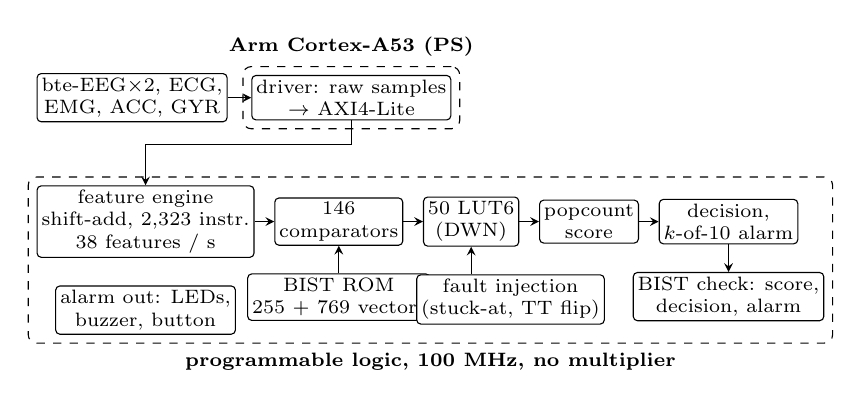
\begin{tikzpicture}[font=\scriptsize, >=stealth,
  blk/.style={draw, rounded corners=1.5pt, align=center, minimum height=5.2mm, inner sep=1.6pt, fill=white},
  grp/.style={draw, dashed, rounded corners=3pt, inner sep=3pt}]
  % Arm side
  \node[blk] (sens) at (0,0) {bte-EEG$\times$2, ECG,\\EMG, ACC, GYR};
  \node[blk, right=3mm of sens] (drv) {driver: raw samples\\$\to$ AXI4-Lite};
  \node[grp, fit=(drv), label={[font=\scriptsize\bfseries]above:Arm Cortex-A53 (PS)}] (ps) {};
  % fabric
  \node[blk, below=8mm of sens.south west, anchor=north west] (fe) {feature engine\\shift-add, 2,323 instr.\\38 features / s};
  \node[blk, right=2.5mm of fe] (cmp) {146\\comparators};
  \node[blk, right=2.5mm of cmp] (lut) {50 LUT6\\(DWN)};
  \node[blk, right=2.5mm of lut] (pop) {popcount\\score};
  \node[blk, right=2.5mm of pop] (alm) {decision,\\$k$-of-10 alarm};
  \node[blk, below=3.5mm of cmp] (rom) {BIST ROM\\255 + 769 vectors};
  \node[blk, below=3.5mm of lut, xshift=5mm] (fi) {fault injection\\(stuck-at, TT flip)};
  \node[blk, below=3.5mm of alm] (chk) {BIST check: score,\\decision, alarm};
  \node[blk, below=3.5mm of fe] (io) {alarm out: LEDs,\\buzzer, button};
  \node[grp, fit=(fe)(alm)(rom)(io)(chk), label={[font=\scriptsize\bfseries]below:programmable logic, 100 MHz, no multiplier}] (pl) {};
  \draw[->] (sens) -- (drv);
  \draw[->] (drv.south) |- ++(0,-3mm) -| (fe.north);
  \draw[->] (fe) -- (cmp);
  \draw[->] (cmp) -- (lut);
  \draw[->] (lut) -- (pop);
  \draw[->] (pop) -- (alm);
  \draw[->] (rom.north) -- (cmp.south);
  \draw[->] (fi.north -| lut.south) -- (lut.south);
  \draw[->] (alm.south) -- (chk.north);
\end{tikzpicture}
}
\caption{Block diagram of SeizeLUT on the Kria KV260, with the fault-injection registers and the self-test that let
the device check that the fabric still computes the validated classifier}\label{fig:arch}
\end{figure}

\section{Hardware Components}

\begin{table}[H]
\centering\small
\caption{Main hardware components}\label{tab:components}
\begin{tabularx}{\textwidth}{|P{30mm}|P{50mm}|L|}
\hline
\multicolumn{1}{|c|}{\textbf{Component}} & \multicolumn{1}{c|}{\textbf{Part / specification}} & \multicolumn{1}{c|}{\textbf{Function}}\\
\hline
FPGA board & AMD Kria KV260 (Zynq UltraScale+ XCK26: four Arm Cortex-A53 cores and FPGA fabric), Ubuntu 22.04 with Kria-PYNQ & Feature engine, classifier, self-test, fault injection, demo outputs\\
\hline
Alarm LED & Red LED with 220\,$\Omega$ resistor on PMOD B1 & Lights while the alarm is on\\
\hline
Buzzer & Buzzer switched by a BC547 transistor (1\,k$\Omega$ base resistor) on PMOD B2 & Sounds while the alarm is on\\
\hline
Alert module & ESP32 Dev Module, USB serial link to the board, alarm wire from PMOD B1 to GPIO\,27 & Push notification and live page on the doctor's phone\\
\hline
Phone & iPhone with the ntfy app; personal hotspot as the network & Receives the alert; ``On my way'' reply\\
\hline
Laptop & Web browser & Live dashboard of the detector\\
\hline
\end{tabularx}
\end{table}

The board runs the detector from recorded test-patient signals stored on it, second by second, exactly as it would
from live sensors. The ESP32 is powered by the USB cable from the board, which also carries the alarm messages; the
alarm wire is a backup that works even if the board's software stops.

\section{Sensor Configuration}

The detector uses the signals of the SeizeIT2 wearable (Table~\ref{tab:modalities}). The two EEG channels are one
behind-the-ear channel and one cross-head channel, chosen per recording by the dataset. A presence bit per sensor
tells the classifier when a sensor is missing.

\begin{table}[H]
\centering\small
\caption{Signals recorded by the wearable (rates measured from the files)}\label{tab:modalities}
\begin{tabular}{|l|l|c|}
\hline
\multicolumn{1}{|c|}{\textbf{Signal}} & \multicolumn{1}{c|}{\textbf{Channels}} & \textbf{Rate}\\
\hline
Behind-the-ear EEG & 2 (left, right or cross-head) & 256 Hz\\
\hline
ECG & 1 & 256 Hz\\
\hline
EMG & 1 & 256 Hz\\
\hline
Motion & 3-axis accelerometer + 3-axis gyroscope & 25 Hz\\
\hline
\end{tabular}
\end{table}

\section{Board Software and Live Demonstration}

\begin{itemize}
\item \textbf{Driver and tests:} a Python driver (PYNQ) with a fast C path writes raw samples and reads results. One
  script (\texttt{run\_board\_tests.sh}) runs nine tests and saves every number to a results file.
\item \textbf{Dashboard:} recorded test-patient signals stream second by second through the board, and a laptop
  browser shows the signals, features, comparator bits, LUT votes, score and alarm, with a check on every window that
  the FPGA equals the software (Figure~\ref{fig:dashboard}, Chapter~\ref{ch:results}).
\item \textbf{Breadboard:} the alarm LED, the buzzer and the ESP32 alarm wire are driven directly by the FPGA pins,
  so they follow the hardware decision.
\end{itemize}

\begin{table}[H]
\centering\small
\caption{Breadboard wiring of the demonstration}\label{tab:wiring}
\begin{tabularx}{\textwidth}{|P{30mm}|L|}
\hline
\multicolumn{1}{|c|}{\textbf{PMOD pin}} & \multicolumn{1}{c|}{\textbf{Connection}}\\
\hline
B1 & 220\,$\Omega$ to the red LED (long leg); short leg to ground; also ESP32 GPIO\,27\\
\hline
B2 & 1\,k$\Omega$ to the BC547 base; emitter to ground; collector to the buzzer ($-$)\\
\hline
B3 (optional) & ESP32 GPIO\,26 (second alarm wire)\\
\hline
3.3\,V & buzzer (+)\\
\hline
GND & ground rail, ESP32 GND\\
\hline
\end{tabularx}
\end{table}

\section{Doctor Alert with an ESP32}\label{sec:alert}

\begin{itemize}
\item \textbf{Board to ESP32:} the board sends one short message per event over USB serial (alarm start, updates
  every 15\,s, escalations, end, patient button).
\item \textbf{ESP32 to phone:} the ESP32 joins the phone's Wi-Fi hotspot, sends a push notification through the ntfy
  service and serves a live alarm page on the same network.
\item \textbf{Phone to board:} the doctor's ``On my way'' reaches the ESP32 and is sent back to the board, where the
  dashboard shows it.
\end{itemize}

The detector answers ``seizure-like or not''; it was not trained to name a seizure type, so the alert reports only
signs that the front end measures, compared with the minute before the alarm (Table~\ref{tab:signs}).

\begin{table}[H]
\centering\small
\caption{The signs in the alert}\label{tab:signs}
\begin{tabularx}{\textwidth}{|l|L|P{45mm}|}
\hline
\multicolumn{1}{|c|}{\textbf{Sign}} & \multicolumn{1}{c|}{\textbf{Shown as}} & \multicolumn{1}{c|}{\textbf{Measured from}}\\
\hline
Heart rate & before and now, NORMAL / HIGH / VERY HIGH & ECG R-peak intervals\\
\hline
Shaking & LITTLE / SOME / STRONG & accelerometer (or gyroscope)\\
\hline
Muscle tension & NORMAL / HIGH & EMG power\\
\hline
Brain activity & MILD / HIGH, slow or fast waves & EEG line length and band power\\
\hline
Pattern hint & ``motor pattern likely'' or ``little movement'' & movement change\\
\hline
\end{tabularx}
\end{table}

Because the doctor has very little time, the alert is designed to be read in about two seconds:

\begin{itemize}
\item \textbf{Notification:} three lines, for example ``SEIZURE Bed 3 / GO TO BED 3 NOW: PROTECT FROM INJURY / Heart
  120 bpm HIGH \textbar{} Shaking STRONG \textbar{} Brain HIGH''.
\item \textbf{Page:} status and a running timer, one instruction, ``On my way'' and ``Call'' buttons, and four colour
  tiles (red = act, amber = watch, green = normal); the emergency plan and first-aid steps are folded below.
\item \textbf{One instruction}, the most urgent first: CHECK BREATHING AND PULSE NOW (heart rate above 150 or below
  40\,bpm, or an unreadable ECG without shaking) $>$ OVER 5 MIN: START EMERGENCY PLAN $>$ OVER 2 MIN: GET EMERGENCY
  PLAN READY $>$ GO TO BED NOW: PROTECT FROM INJURY (strong shaking) $>$ GO TO BED NOW. When it ends: SEIZURE STOPPED:
  CHECK BREATHING, TURN ON SIDE.
\item \textbf{Escalation} at 2 and 5 minutes of alarm, then every minute; five minutes is the ILAE time point for
  treating a convulsive seizure as status epilepticus. \textbf{Reminders} every minute until someone taps ``On my
  way''; \textbf{clusters} (``2nd seizure this hour'') are flagged; only a bed name is sent, never a patient name.
\end{itemize}

The movement-based pattern hint was checked against the doctors' motor and non-motor labels of the 702 seizures of
the training patients only. In the first 30\,s movement rose 4.8-fold (median) in motor seizures and 1.04-fold in
non-motor seizures. A threshold (2.6-fold) chosen on patients 1--48 matched the doctors' label on patients 49--96 in
64\,\% of cases (balanced accuracy; 48\,\% of motor and 79\,\% of non-motor seizures), so the hint is useful but is not
a diagnosis.

\chapter{SIGNAL PROCESSING AND CLASSIFICATION METHODOLOGY}\label{ch:method}

\section{Dataset}

SeizeIT2 \cite{bhagubai2025seizeit2} (OpenNeuro ds005873 v1.1.0, CC0) holds wearable recordings of 125 patients with
focal epilepsy from five European epilepsy units, with seizures annotated on hospital video-EEG. We use the official
split: \textbf{96 training patients} for all development and \textbf{29 test patients} (sub-097 to sub-125) scored
once, after the design was frozen. Table~\ref{tab:inventory} and Figures~\ref{fig:classes} and~\ref{fig:hours}
summarise the dataset; all values were measured by our audit.

\begin{table}[H]
\centering\small
\caption{Inventory of SeizeIT2 measured by our audit}\label{tab:inventory}
\begin{tabular}{|l|l|}
\hline
\multicolumn{1}{|c|}{\textbf{Quantity}} & \multicolumn{1}{c|}{\textbf{Value}}\\
\hline
Patients / recordings / EDF files & 125 / 2,850 / 11,009 (125.9 GB)\\
\hline
Hours of EEG & 11,626 h (median 95 h per patient)\\
\hline
Seizures & 883 (train 702, test 181)\\
\hline
Seizure time & 14.3 h = \textbf{0.123\,\%} of the recording time\\
\hline
Seizure duration & 2--962 s (median 33 s)\\
\hline
Missing ECG/EMG; missing motion & 3.1\,\%; 3.9\,\% of the time\\
\hline
\end{tabular}
\end{table}

\begin{figure}[H]
\centering
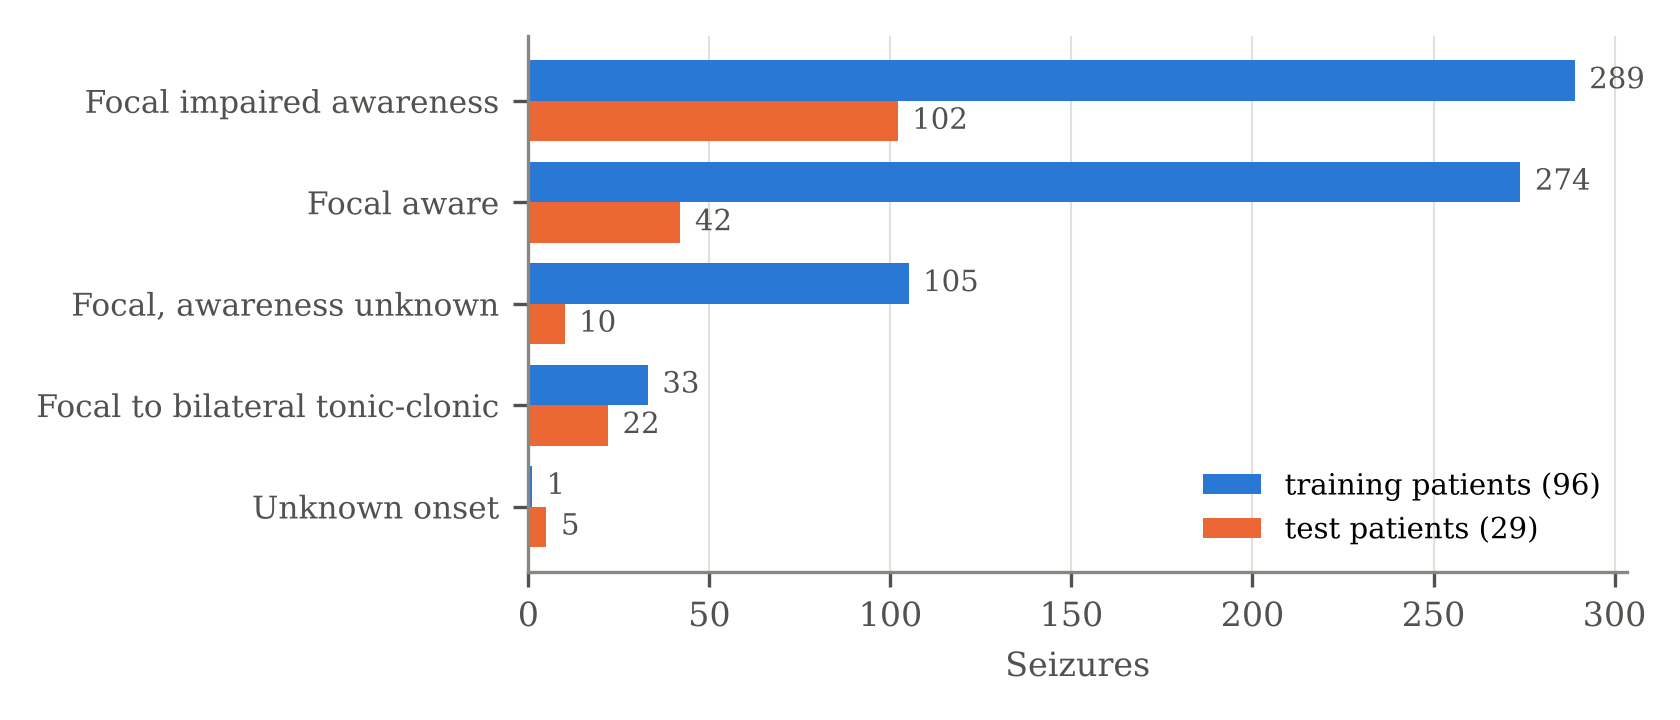
\includegraphics[width=0.78\textwidth]{figures/seizure_classes.png}
\caption{Seizure classes in the training and test patients: 822 of 883 seizures are focal seizures that do not become
tonic-clonic}\label{fig:classes}
\end{figure}

\begin{figure}[H]
\centering
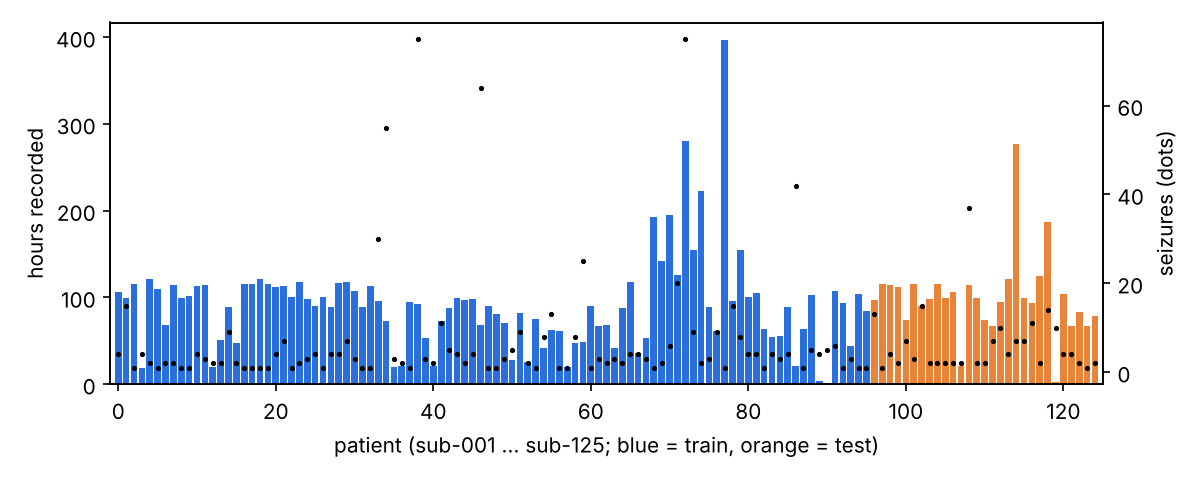
\includegraphics[width=0.9\textwidth]{figures/hours_and_seizures_per_patient.png}
\caption{Hours recorded (bars; blue: training, orange: test) and seizures per patient (dots)}\label{fig:hours}
\end{figure}

\section{Audit Findings}

\begin{table}[H]
\centering\small
\caption{Where the released files differ from the documentation, and what we did}\label{tab:docdiff}
\begin{tabularx}{\textwidth}{|P{34mm}|P{25mm}|P{30mm}|L|}
\hline
\multicolumn{1}{|c|}{\textbf{Item}} & \multicolumn{1}{c|}{\textbf{Documentation}} & \multicolumn{1}{c|}{\textbf{Files}} & \multicolumn{1}{c|}{\textbf{Action}}\\
\hline
Sampling rate & 250 Hz & 256 Hz & Filters designed for 256 Hz\\
\hline
Seizures & 886 & 883 & Report our count\\
\hline
Centre and age labels & used for splits & not released & Folds by seizure count\\
\hline
Official artefact rule & 13--150\,\textmu V & flags 69\,\% of normal windows & Flags used as input bits\\
\hline
Downloads & -- & 9 files cut short & Size checks; re-extracted\\
\hline
Evaluation code & -- & two defects & Corrected values reported alongside\\
\hline
\end{tabularx}
\end{table}

\section{Development Pipeline}

\begin{figure}[H]
\centering
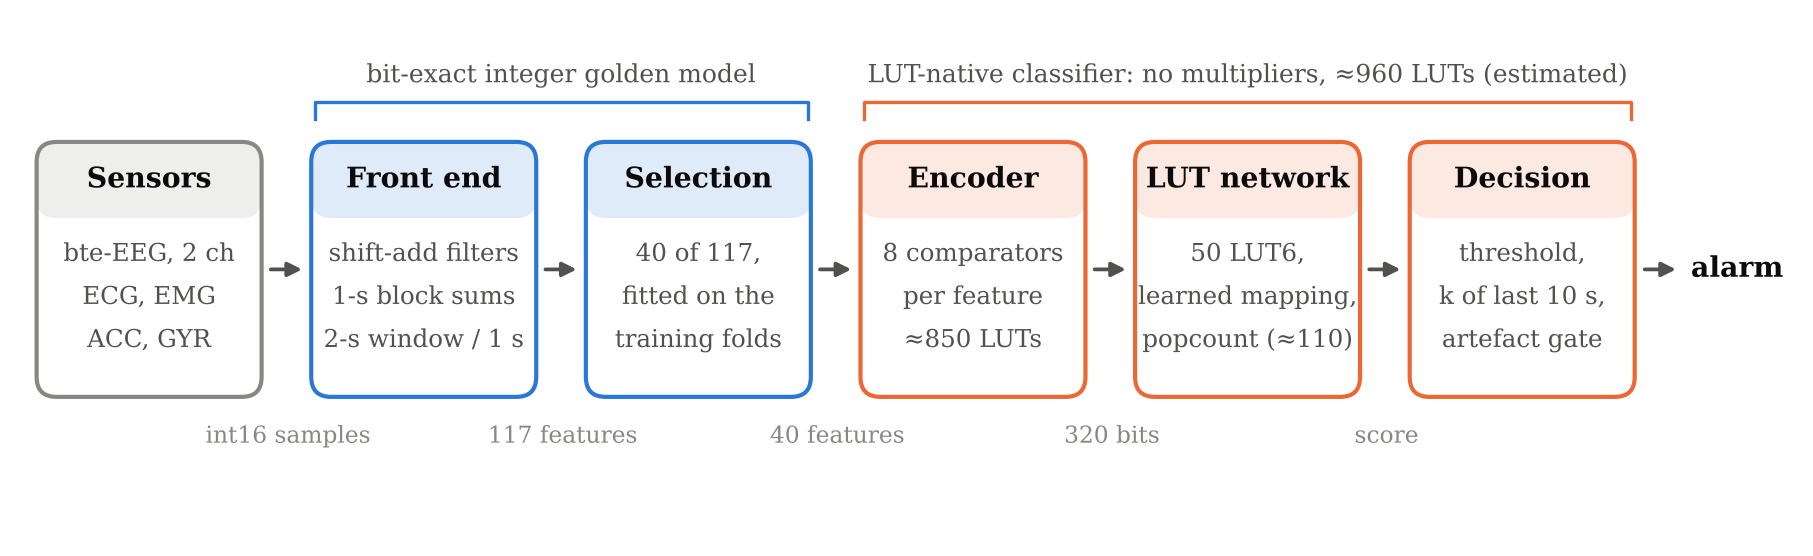
\includegraphics[width=\textwidth]{figures/system_overview.png}
\caption{Development pipeline of the detector. Blue: bit-exact integer front end; orange: LUT-native classifier (the
LUT count is the estimate for the base network)}\label{fig:system}
\end{figure}

\begin{enumerate}
\item Every second, the last 2\,s of all signals become \textbf{117 integer features} (Table~\ref{tab:features}).
\item The most useful features are thermometer-encoded (each feature compared with learned thresholds) and classified
  by a \textbf{50-LUT network}. In the final, distilled network the 50 LUTs read \textbf{146 threshold bits} from
  \textbf{38 features}; only these comparators are built in hardware.
\item The 50 LUT outputs are counted into a score, and an alarm is raised when the score is high in 10 of the last
  10 seconds.
\end{enumerate}

\section{Integer Front End and Feature Sets}

\begin{table}[H]
\centering\small
\caption{The 117 integer features (per 2-s window; many also as change from a 64-s moving average)}\label{tab:features}
\begin{tabularx}{\textwidth}{|l|c|L|}
\hline
\multicolumn{1}{|c|}{\textbf{Group}} & \textbf{Count} & \multicolumn{1}{c|}{\textbf{Features}}\\
\hline
EEG & 84 & amplitude, line length, mobility, zero crossings, extrema, 5 band amplitudes; artefact flags\\
\hline
ECG & 5 & log heart period, log RR variability, quality flag\\
\hline
EMG & 8 & amplitude, line length, zero crossings, high/low band ratio\\
\hline
Motion & 16 & accelerometer and gyroscope magnitude, jerk, activity, band amplitude\\
\hline
Presence & 4 & one bit per sensor (ECG, EMG, accelerometer, gyroscope)\\
\hline
\end{tabularx}
\end{table}

\textbf{Integer arithmetic.} Every filter coefficient is a sum of a few signed powers of two, so filtering needs only
shifts and additions, and error feedback keeps the rounding noise below one least significant bit. Heart rate is
represented by $\log_2(\mathrm{RR})$, so there is no division. The same front end exists in Python (the golden model),
in C (on the Arm and in the demo) and as a microcoded engine in the FPGA fabric (Chapter~\ref{ch:hw}), and all three
give the same integers for every window. A floating-point twin measures the cost of the integer arithmetic
(Section~\ref{sec:verif}).

\section{LUT-Native Classifier (DWN)}

A Differentiable Weightless Neural Network \cite{bacellar2024dwn} has no weights: each neuron is a 6-input truth table,
exactly one FPGA LUT.
\begin{equation}
  b_{f,i} = [\,x_f > t_{f,i}\,] \qquad\qquad s = \sum_{j \in S} y_j - \sum_{j \in B} y_j
\end{equation}
Each threshold bit $b_{f,i}$ is one comparator; each neuron reads 6 learned bits and outputs one stored bit $y_j$; the
score $s$ is the popcount of the seizure group $S$ minus that of the background group $B$. The network is trained by
gradient descent through a differentiable relaxation of the lookup, and in the final version by distillation from a
LightGBM teacher. The trained truth tables are loaded straight into the FPGA's LUT6 elements.

\section{Models and Extensions}

\begin{table}[H]
\centering\small
\caption{Models compared on the same features, splits and metrics}\label{tab:models}
\begin{tabularx}{\textwidth}{|P{36mm}|L|}
\hline
\multicolumn{1}{|c|}{\textbf{Group}} & \multicolumn{1}{c|}{\textbf{Models}}\\
\hline
Published baselines & ChronoNet \cite{roy2019chrononet} (CNN + GRU on raw EEG); SVM \cite{vandecasteele2020bte}\\
\hline
Software references & logistic regression, random forest, XGBoost, LightGBM, CatBoost\\
\hline
Hardware-oriented & INT8 MLP (multipliers), TreeLUT \cite{khataei2025treelut}, logic-gate network \cite{petersen2022dlgn}, DWN \cite{bacellar2024dwn}\\
\hline
\end{tabularx}
\end{table}

\begin{table}[H]
\centering\small
\caption{Extensions of the DWN tested in this project (adopted only if significantly better)}\label{tab:extensions}
\begin{tabularx}{\textwidth}{|c|L|}
\hline
\textbf{ID} & \multicolumn{1}{c|}{\textbf{Idea}}\\
\hline
N1 & Memory across seconds: 16 state bits fed back; stacked past windows\\
\hline
N2 & Encoder design: uniform, Gaussian and learned thresholds\\
\hline
N3 & Label-free per-patient threshold adaptation\\
\hline
N4 & Distillation from LightGBM; teacher-guided hard negatives\\
\hline
N5 & Focal, noise-robust (GCE, SCE) and multiple-instance losses; onset weighting\\
\hline
N6 & Modality dropout, gated fusion, late fusion\\
\hline
N7 & Interpretability: which inputs the LUTs read during alarms\\
\hline
N8 & Post-ictal verification: a second LUT network confirms each alarm (secondary analysis)\\
\hline
N9 & Fault analysis and self-test of the LUT network\\
\hline
N10 & Front end in the FPGA fabric (microcoded shift-add engine)\\
\hline
\end{tabularx}
\end{table}

\section{Evaluation Protocol}\label{sec:eval}

\begin{itemize}
\item \textbf{Patient-wise 5-fold cross-validation} on the 96 training patients for every design choice.
\item \textbf{Sealed test set}: the 29 test patients scored once, after the freeze, with 5 seeds; every access logged.
\item \textbf{SzCORE event scoring} \cite{dan2024szcore} (30\,s before, 60\,s after, 90\,s merge), per patient:
\end{itemize}
\begin{equation}
  \mathrm{Sens} = \frac{TP}{TP + FN},\qquad \mathrm{Prec} = \frac{TP}{TP + FP},\qquad
  F_1 = \frac{2\,\mathrm{Sens}\cdot\mathrm{Prec}}{\mathrm{Sens} + \mathrm{Prec}},\qquad \text{false alarms per 24 h}
\end{equation}
\begin{itemize}
\item \textbf{Operating points} (threshold, $k$, artefact gate) chosen on the training folds: best event-F1, and highest
  sensitivity with at most one false alarm per hour.
\item \textbf{Statistics}: paired Wilcoxon test per patient; an extension is adopted only if $p < 0.05$ in its favour.
\item \textbf{Paper metrics} (the base paper's own code) are reported for the comparison with the base paper.
\item \textbf{Compute}: a 4-core CPU server and a laptop RTX 3060 GPU.
\end{itemize}

\chapter{HARDWARE IMPLEMENTATION OF THE DETECTOR}\label{ch:hw}

\section{Design and Interface}

The detector is one IP core inside the KV260 design (core version 3). It is reached through one AXI4-Lite slave at
100\,MHz with an 8-KB window: control and result registers, the feature registers, and the feature engine's register
file at address 0x1000 (Table~\ref{tab:core}).

\begin{table}[H]
\centering\small
\caption{Blocks of the SeizeLUT core}\label{tab:core}
\begin{tabularx}{\textwidth}{|P{34mm}|L|}
\hline
\multicolumn{1}{|c|}{\textbf{Block}} & \multicolumn{1}{c|}{\textbf{Function}}\\
\hline
Feature engine & Computes the 38 features from raw samples (Section~\ref{sec:fe-engine})\\
\hline
Classifier & 146 threshold comparators, 50 LUT6, popcount score, frozen and programmable operating points, 10-of-10
alarm; latency 3 clock cycles\\
\hline
Self-test (BIST) & Vector ROM and response check; 1,024 vectors in 1,028 cycles\\
\hline
Fault injection & Registers that flip any truth-table bit or force any comparator or LUT output to 0 or 1\\
\hline
Debug read-back & All 146 comparator bits and 50 LUT outputs of the last window\\
\hline
Demo I/O & PMOD outputs for the alarm LED, buzzer, score LEDs and a heartbeat; a debounced button input\\
\hline
\end{tabularx}
\end{table}

\section{Feature Engine in the Fabric}\label{sec:fe-engine}

A front end with dozens of filters would need many multipliers if built directly. Instead, a small microcoded
\emph{feature engine} computes the 38 features the classifier reads, one instruction at a time:

\begin{itemize}
\item one 40-bit adder and two 5-bit shifters; every filter coefficient is a sum of at most five signed powers of
  two, so a multiplication becomes a few shifted additions;
\item a register file of 930 words and a 2,323-instruction program in block RAM, at 3 clock cycles per instruction;
\item four events: a 256-Hz biopotential sample, a 25-Hz motion sample, the end of a second, and the last window.
\end{itemize}

After each window the core copies the engine's 38 features into the classifier and classifies them automatically. The
engine needs under one million cycles per second of signal, so it keeps up with the sensors at 1\,MHz, a hundredth of
the board's clock.

\section{Operation and Verification}

\begin{enumerate}
\item The Arm writes the raw samples of one second into the engine's register file and starts the events.
\item The engine runs its program and writes the 38 features; the core copies them into the classifier registers.
\item The comparators, the 50 LUTs and the popcount produce the score, the decision and the alarm in 3 cycles.
\item The Arm reads the result; the LED, buzzer and ESP32 wire follow the alarm bit directly.
\end{enumerate}

Every stage was verified against the software model before the board build: the engine program in an
instruction-level simulator, the engine RTL sample by sample and the whole core through the AXI bus in Verilator
(Section~\ref{sec:verif}).

\section{Built-In Self-Test}\label{sec:bist}

\textbf{Fault model.} Every single fault in the part of the hardware the network adds: each of the $50 \times 64 =
3{,}200$ truth-table bits flipped (an upset in FPGA configuration memory) and each comparator and LUT output stuck at 0
or 1 (292 + 100), 3,592 faults in total.

\textbf{Which faults matter.} Each fault was applied to all 31.4 million windows (8,714 hours) of the 96 training
patients. A fault is \emph{decision-relevant} if it changes at least one decision, and \emph{alarm-relevant} if it
changes at least one alarm.

\textbf{Test vectors.} 255 test vectors were chosen from training windows for coverage, so that together they
exercise every decision-relevant fault. The on-chip self-test runs 1,024 vectors in 1,028 clock cycles
(10.3\,\textmu s), so the device can test itself after every one-second window. The detection results are in
Section~\ref{sec:res-bist}.

\chapter{RESULTS}\label{ch:results}

Sections~\ref{sec:verif}--\ref{sec:res-dev} cover development on the 96 training patients (patient-wise
cross-validation) and the verification of every implementation. Sections~\ref{sec:res-test}--\ref{sec:res-n8} cover
the single evaluation on the 29 held-out test patients after the design was frozen. Sections~\ref{sec:res-fpga}--%
\ref{sec:res-demo} cover the FPGA and the board.

\section{Verification of the Implementation}\label{sec:verif}

\begin{table}[H]
\centering\small
\caption{Verification of the integer front end and of the hardware}\label{tab:verif}
\begin{tabularx}{\textwidth}{|L|P{62mm}|}
\hline
\multicolumn{1}{|c|}{\textbf{Check}} & \multicolumn{1}{c|}{\textbf{Result}}\\
\hline
Integer features against the floating-point twin (10 training patients) & median correlation 0.9965; artefact flags
agree 99.7\,\%; LightGBM AUROC 0.736 vs 0.735\\
\hline
Verilog of the final DWN against the software (Icarus Verilog, 10 test recordings) & 431,960 windows, 0 mismatches
(features, bits, LUT outputs, scores, alarms)\\
\hline
Engine program (instruction-level simulator) against the C front end, 10 recordings & all 431,960 windows equal (38
features)\\
\hline
Engine RTL fed sample by sample (Verilator), EEG-only and all-sensor recording & 4,278 windows, 0 mismatches\\
\hline
Whole core from raw samples through AXI (Verilator) & 4,278 windows: features, score, decision and alarm equal\\
\hline
Whole core RTL regression with every fault injected & 863,920 checks and all 3,592 faults pass\\
\hline
\end{tabularx}
\end{table}

\section{Reproduction of the Published Baseline}\label{sec:res-chrononet}

\begin{figure}[H]
\centering
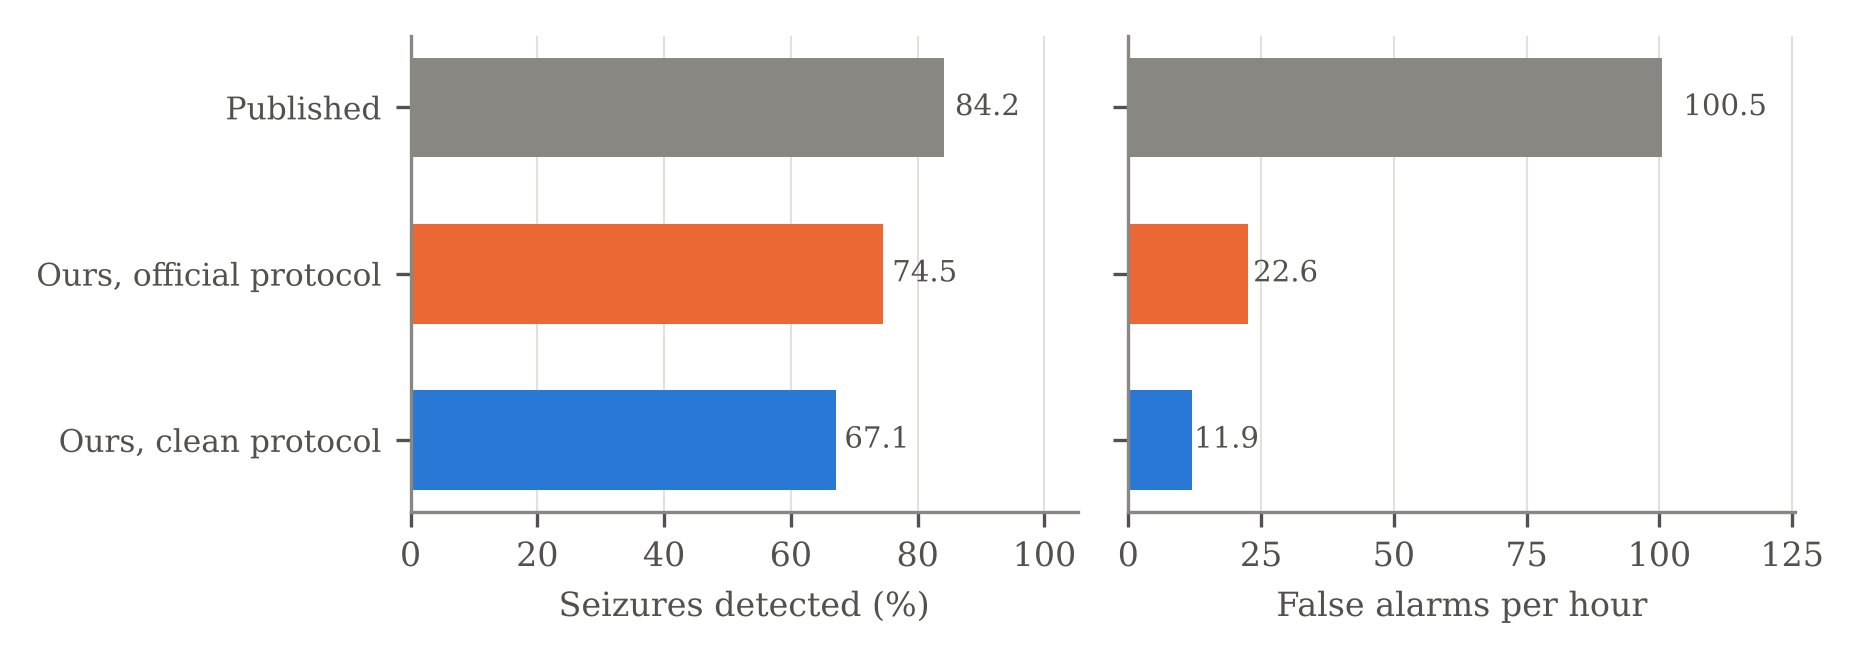
\includegraphics[width=0.9\textwidth]{figures/chrononet_repro.png}
\caption{ChronoNet on the 29 test patients: published and reproduced (the paper's metrics)}\label{fig:chrononet}
\end{figure}

\begin{itemize}
\item \textbf{Partly reproduced}: 74.5\,\% of seizures detected against 84.2\,\% published, with 22.6 instead of 100.5
  false alarms per hour (Figure~\ref{fig:chrononet}); the per-recording AUPR matches (0.109 vs 0.104).
\item \textbf{Test-set leak}: the released code picks its training epoch on the test patients. Our \textbf{clean} run
  (last epoch, no test information: 67.1\,\%, 11.9 false alarms per hour) is the reference for the final comparison.
\end{itemize}

\section{Model Development on the Training Patients}\label{sec:res-dev}

\begin{table}[H]
\centering\small
\caption{Five-fold cross-validation on the 96 training patients (best-F1 operating point)}\label{tab:families}
\setlength{\tabcolsep}{3pt}
\begin{tabularx}{\textwidth}{|P{36mm}|c|c|c|c|L|}
\hline
\multicolumn{1}{|c|}{\textbf{Model}} & \textbf{AUROC} & \textbf{Event-F1} & \textbf{FA/24\,h} & \textbf{Sens.\ $\le$1 FA/h} & \multicolumn{1}{c|}{\textbf{Estimated cost}}\\
\hline
LightGBM & 0.870 & 0.292 & 3.6 & 0.594 & $\approx$30.6k LUTs\\
\hline
CatBoost & 0.863 & 0.286 & 3.0 & 0.618 & $\approx$27.7k LUTs\\
\hline
XGBoost & 0.867 & 0.277 & 3.4 & 0.603 & $\approx$47.9k LUTs\\
\hline
TreeLUT & 0.857 & 0.266 & 4.2 & 0.619 & $\approx$6.4k LUTs\\
\hline
\textbf{DWN + distillation (final)} & 0.851 & \textbf{0.229} & \textbf{0.9} & 0.597 & \textbf{$\approx$870 LUTs}\\
\hline
DWN base & 0.840 & 0.211 & 2.4 & 0.581 & $\approx$960 LUTs\\
\hline
Random forest & 0.852 & 0.198 & 0.5 & 0.536 & $\approx$323k LUTs\\
\hline
Logic-gate network & 0.843 & 0.171 & 4.9 & 0.540 & $\approx$7.5k LUTs\\
\hline
INT8 MLP & 0.830 & 0.147 & 7.8 & 0.520 & 9,600 multiplications\\
\hline
Logistic regression & 0.806 & 0.105 & 8.8 & 0.409 & 117 multiplications\\
\hline
\end{tabularx}
\end{table}

The DWN is 7--8$\times$ smaller than the other LUT models and beats the INT8 MLP on every metric. Larger networks (up
to 2,000 LUTs), 16 thresholds, two layers and other temperatures gave no significant gain (Figure~\ref{fig:pareto});
4-input LUTs and 4 thresholds were clearly worse.

\begin{figure}[H]
\centering
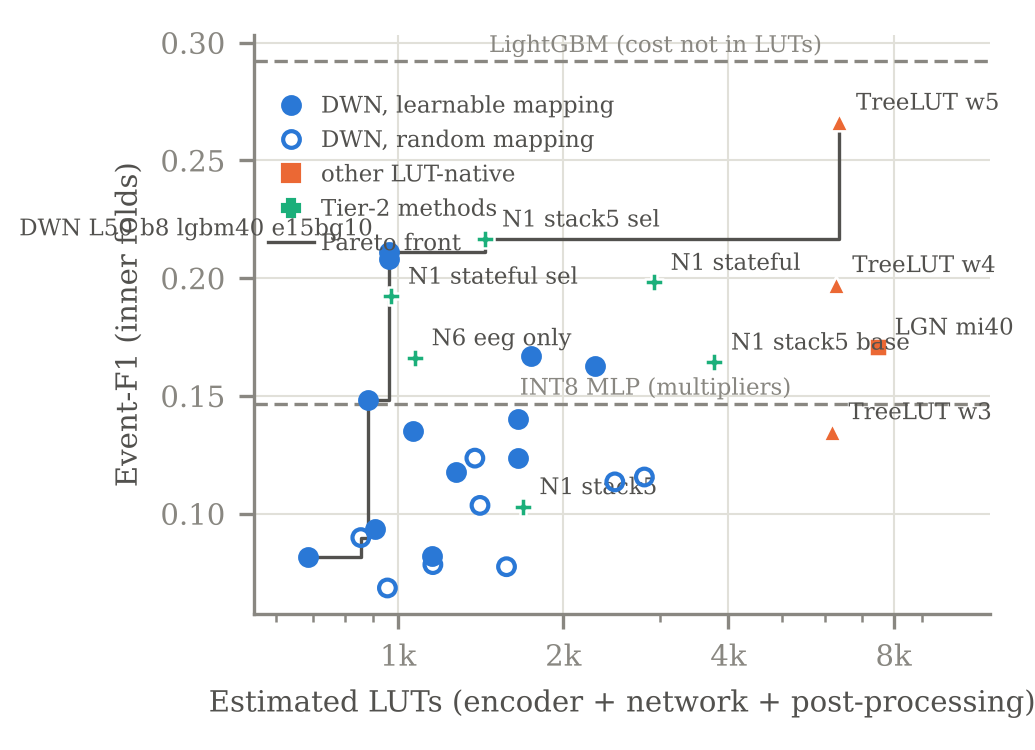
\includegraphics[width=0.66\textwidth]{figures/pareto_inner_cv.png}
\caption{Event-F1 against estimated LUTs for every LUT-native run (training folds), with the Pareto front}\label{fig:pareto}
\end{figure}

\begin{figure}[H]
\centering
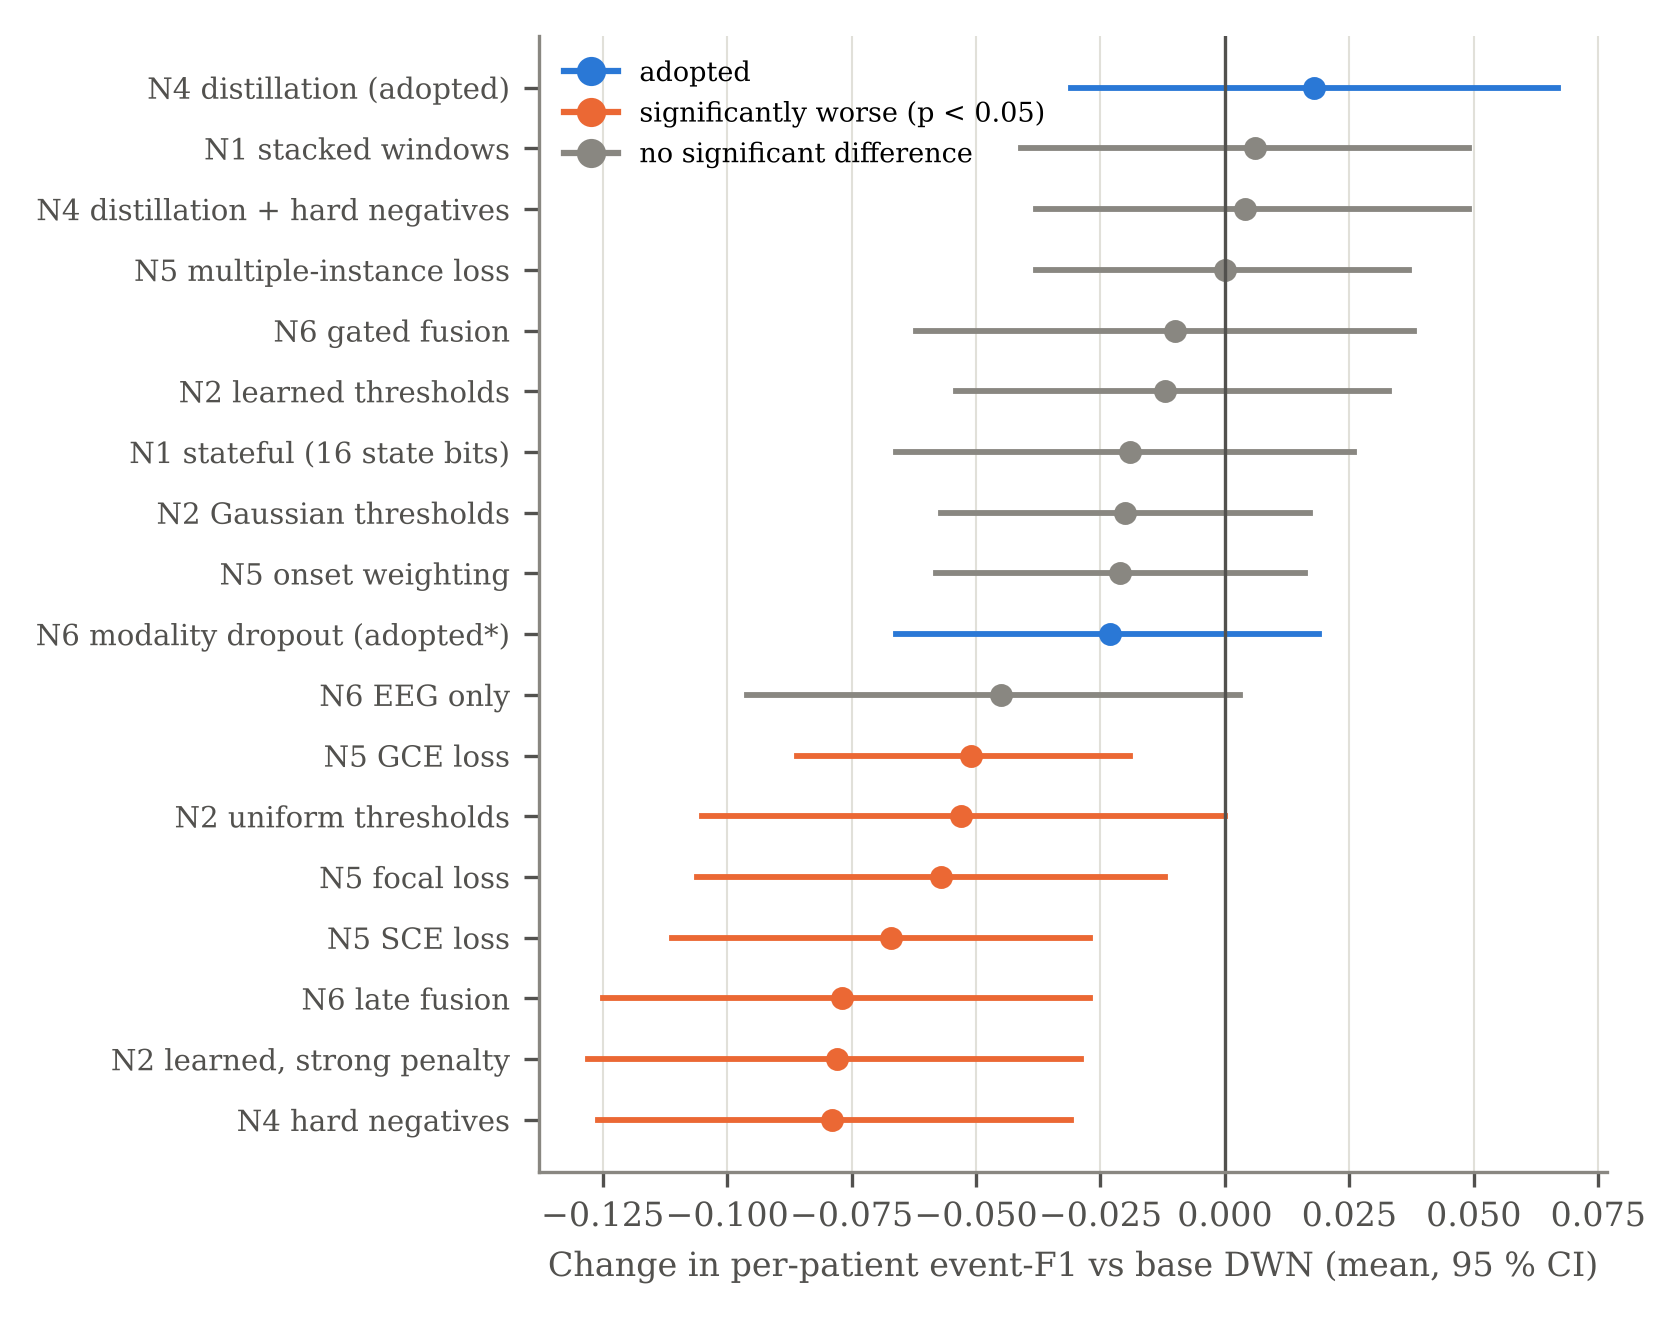
\includegraphics[width=0.85\textwidth]{figures/ablation.png}
\caption{Every extension against the base DWN: mean change in per-patient event-F1 with 95\,\% interval (modality
dropout was adopted for its robustness to missing sensors)}\label{fig:ablation}
\end{figure}

\begin{table}[H]
\centering\small
\caption{The changes that passed the significance test}\label{tab:adopted}
\begin{tabularx}{\textwidth}{|P{40mm}|L|P{34mm}|}
\hline
\multicolumn{1}{|c|}{\textbf{Change}} & \multicolumn{1}{c|}{\textbf{Evidence (training patients)}} & \multicolumn{1}{c|}{\textbf{How it was found}}\\
\hline
Feature selection by LightGBM importance & event-F1 0.148 $\to$ 0.208 ($p = 0.047$); false alarms 7.0 $\to$ 2.3/day & N7 showed the network ignored heart rate\\
\hline
Distillation from LightGBM (\textbf{final}) & false alarms 2.4 $\to$ 0.9/day ($p = 3\times10^{-7}$); event-F1 0.229 vs 0.211 & N4\\
\hline
Modality dropout (variant) & without ECG: event-F1 0.092 $\to$ 0.172 ($p = 0.005$) & N6\\
\hline
\end{tabularx}
\end{table}

\begin{figure}[H]
\centering
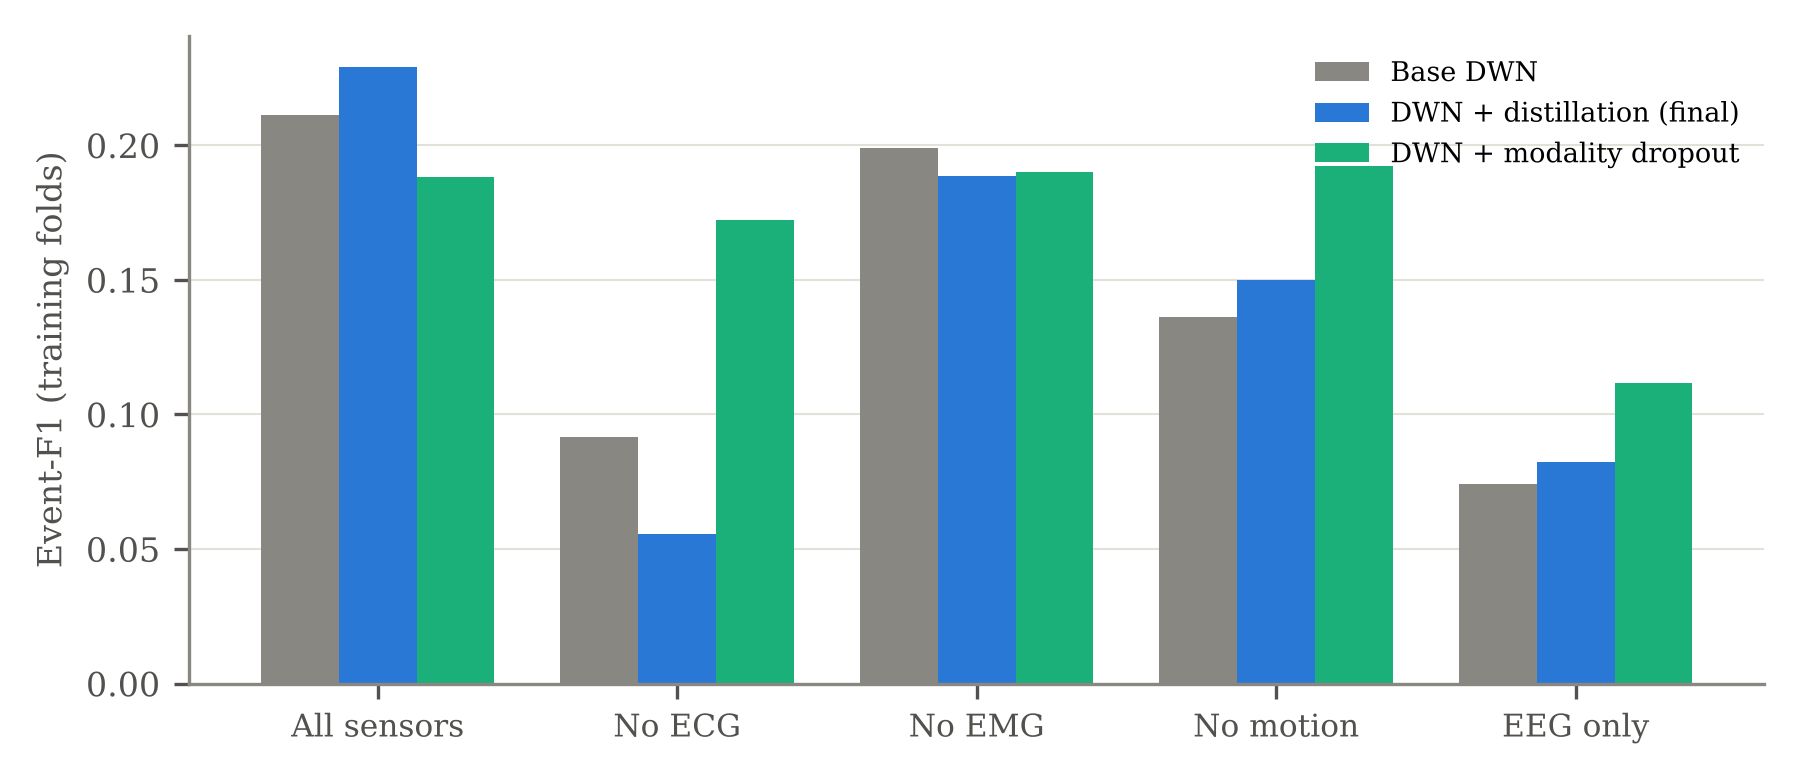
\includegraphics[width=0.85\textwidth]{figures/missing_sensors.png}
\caption{Event-F1 with sensors removed at test time (training folds): distillation is the most accurate with all
sensors; modality dropout keeps working without ECG or motion}\label{fig:missing}
\end{figure}

\begin{figure}[H]
\centering
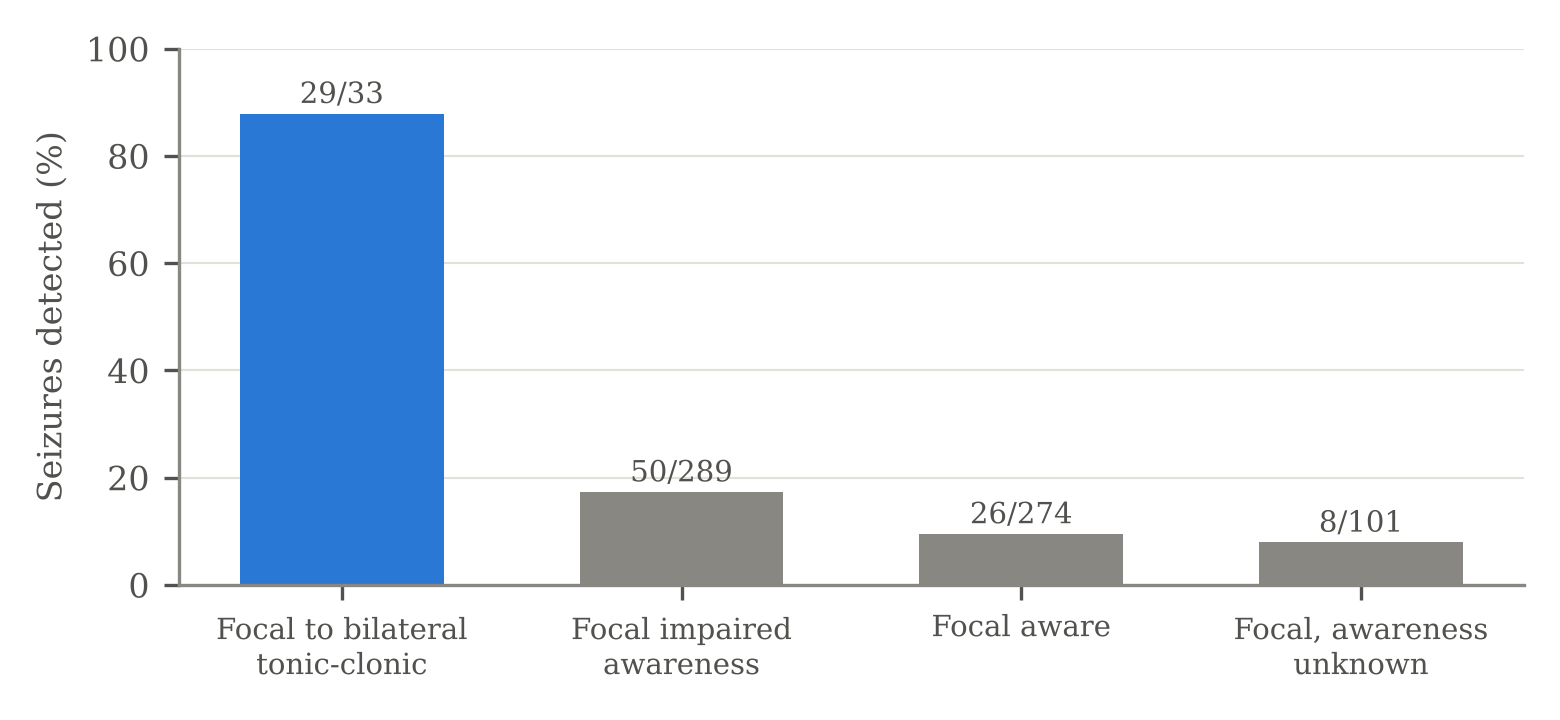
\includegraphics[width=0.62\textwidth]{figures/seizure_types.png}
\caption{Seizures detected by type (base DWN, training folds): tonic-clonic seizures are caught, focal seizures
rarely}\label{fig:types}
\end{figure}

\section{Final Evaluation on the Held-Out Test Patients}\label{sec:res-test}

\begin{figure}[H]
\centering
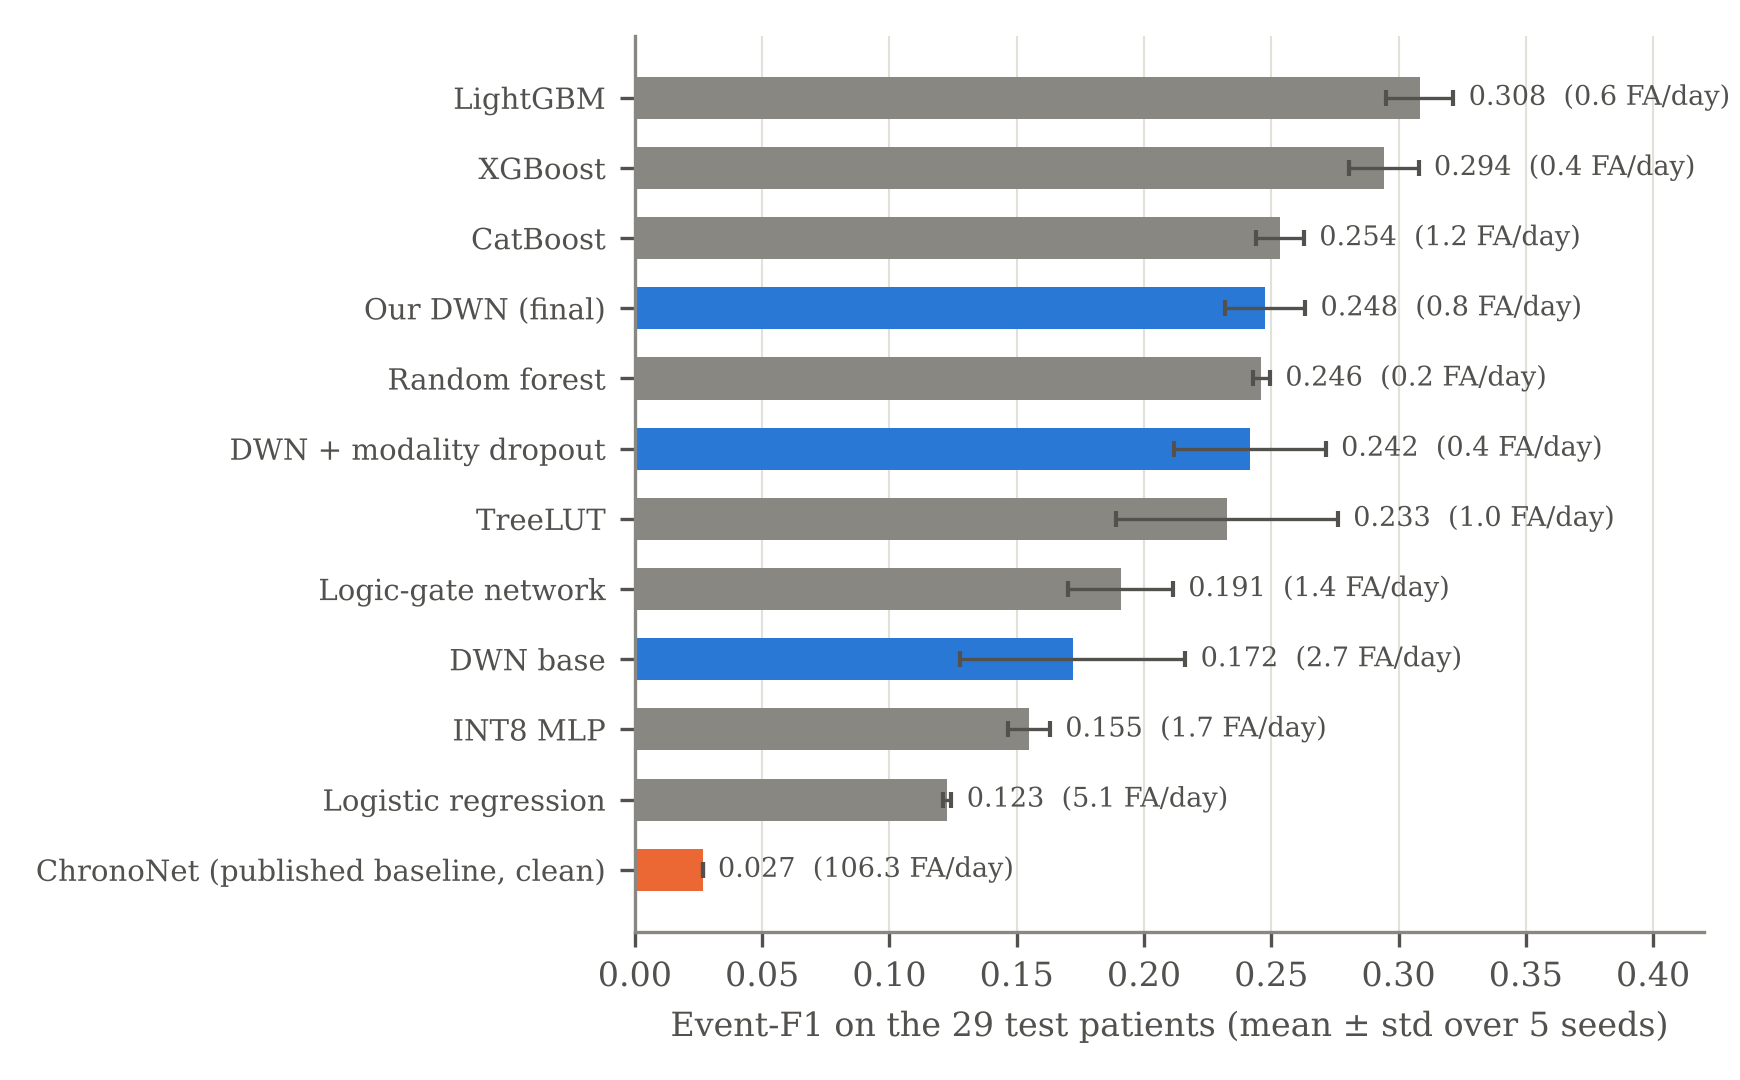
\includegraphics[width=0.85\textwidth]{figures/test_f1.png}
\caption{Event-F1 on the 29 test patients (mean $\pm$ std over 5 seeds) and false alarms per day}\label{fig:testf1}
\end{figure}

\begin{table}[H]
\centering\small
\caption{Final DWN against the main references on the 29 test patients ($p$: paired Wilcoxon on per-patient event-F1)}\label{tab:test}
\begin{tabularx}{\textwidth}{|P{40mm}|c|c|c|L|}
\hline
\multicolumn{1}{|c|}{\textbf{Model}} & \textbf{Event-F1} & \textbf{FA/24\,h} & \textbf{$p$ vs ChronoNet} & \multicolumn{1}{c|}{\textbf{Estimated cost}}\\
\hline
\textbf{DWN + distillation (final)} & \textbf{0.248 $\pm$ 0.016} & \textbf{0.8} & 0.027 & \textbf{$\approx$900 LUTs}\\
\hline
LightGBM & 0.308 $\pm$ 0.013 & 0.6 & 0.027 & $\approx$30.8k LUTs\\
\hline
CatBoost & 0.254 $\pm$ 0.009 & 1.2 & 0.031 & $\approx$27.7k LUTs\\
\hline
Random forest & 0.246 $\pm$ 0.003 & 0.2 & 0.27 & $\approx$347k LUTs\\
\hline
TreeLUT & 0.233 $\pm$ 0.044 & 1.0 & 0.016 & $\approx$6.3k LUTs\\
\hline
Logic-gate network & 0.191 $\pm$ 0.021 & 1.4 & 0.034 & $\approx$7.5k LUTs\\
\hline
INT8 MLP & 0.155 $\pm$ 0.008 & 1.7 & 0.017 & 9,600 multiplications\\
\hline
ChronoNet (clean) & 0.027 & 106 & -- & CNN + GRU\\
\hline
\end{tabularx}
\end{table}

The result held on unseen patients (0.248, above the cross-validation value of 0.229). The final DWN scores above
TreeLUT, the logic-gate network and the INT8 MLP, is level with random forest and CatBoost at 30--390$\times$ fewer
LUTs, and is significantly better than ChronoNet; LightGBM remains ahead ($p = 0.039$). All models are listed in
Appendix~\ref{app:results}.

\begin{figure}[H]
\centering
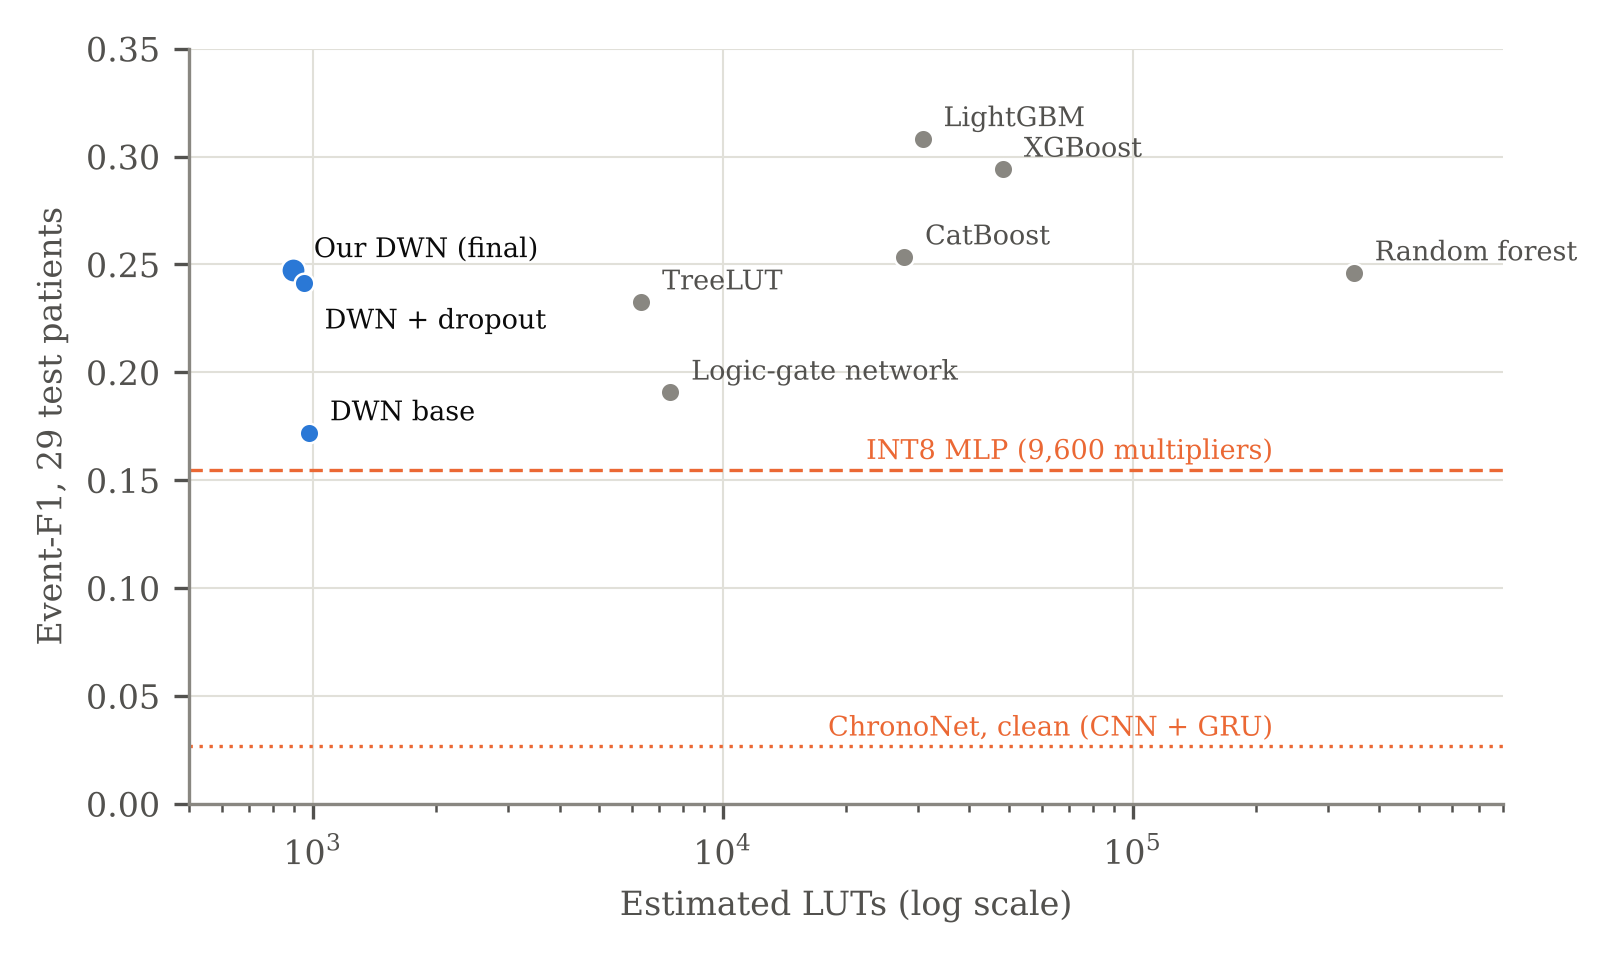
\includegraphics[width=0.78\textwidth]{figures/test_f1_vs_luts.png}
\caption{Accuracy against hardware cost on the test patients: the LUT networks reach tree-ensemble accuracy at a
fraction of the LUTs}\label{fig:testluts}
\end{figure}

\section{Comparison with the Base Paper}\label{sec:res-published}

\begin{figure}[H]
\centering
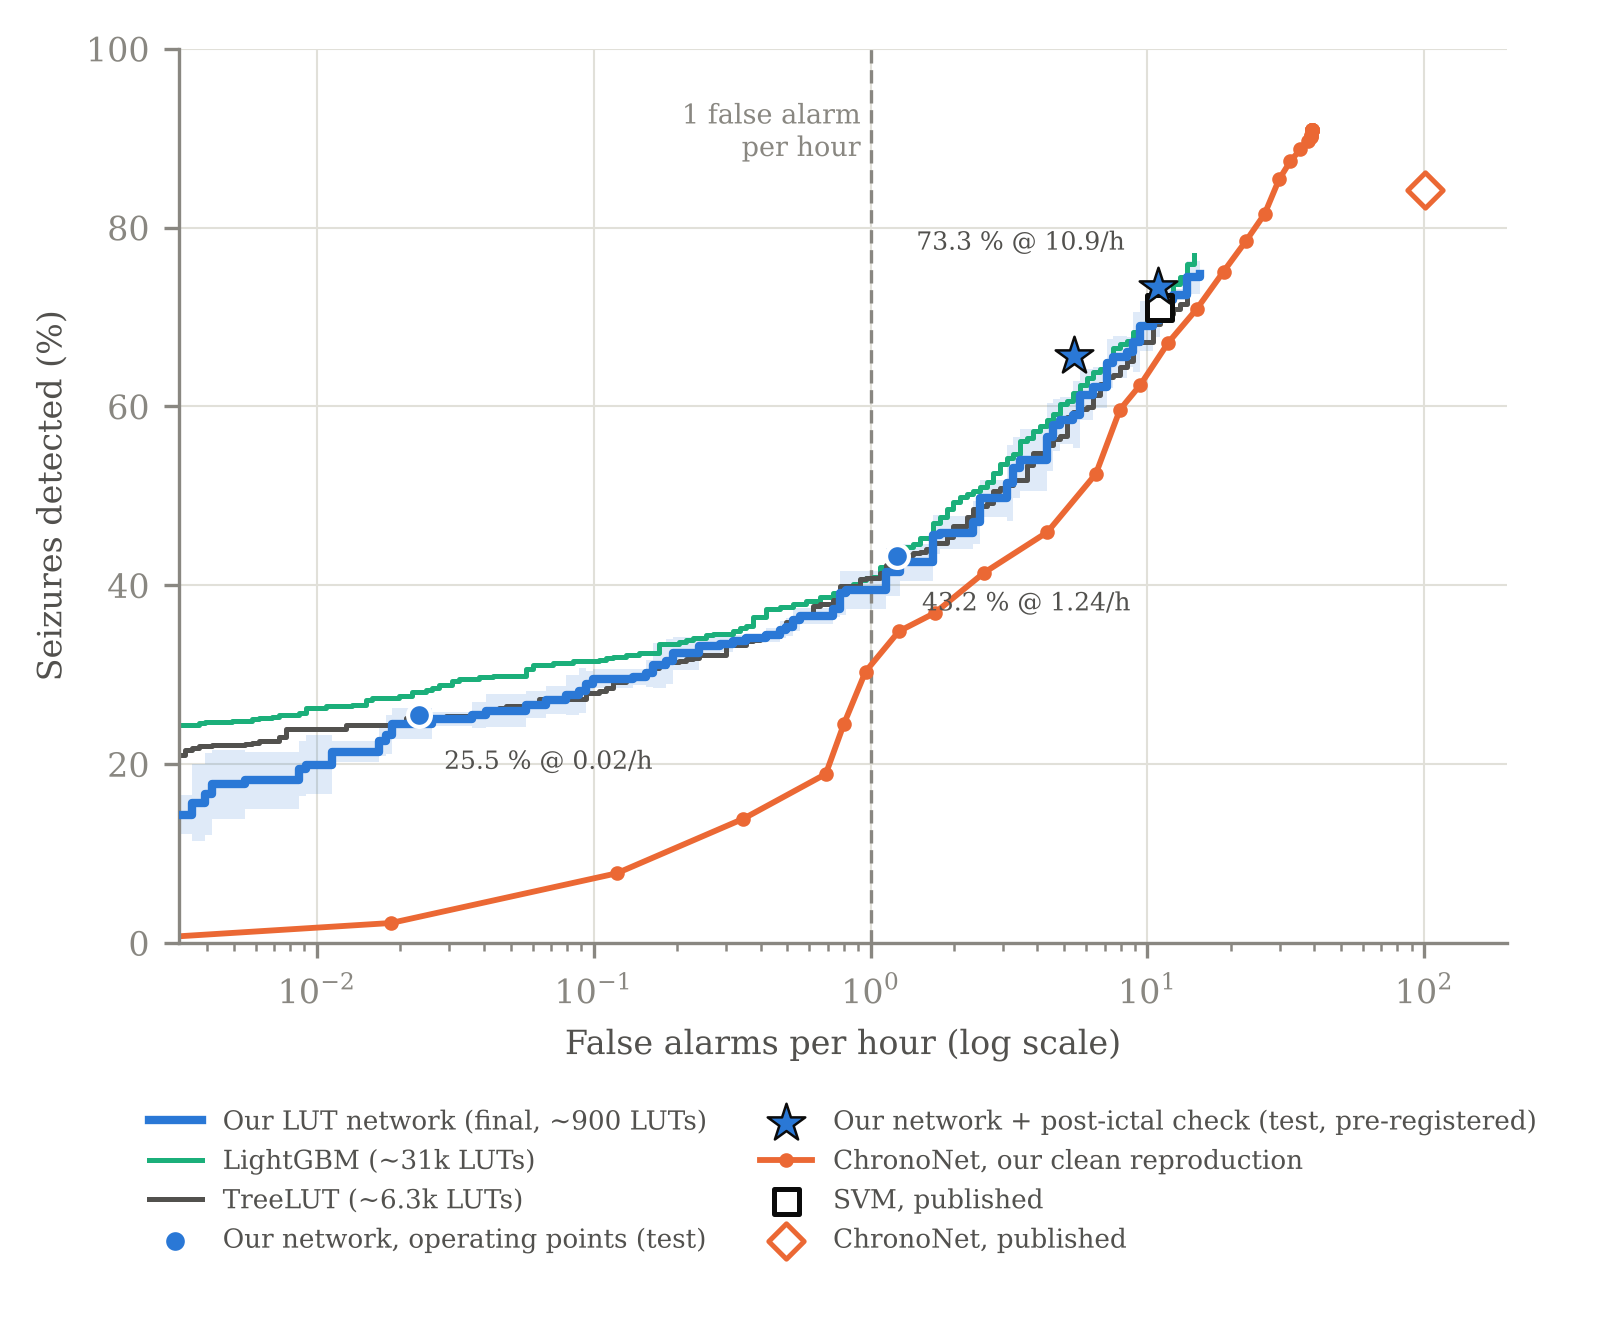
\includegraphics[width=0.82\textwidth]{figures/sens_fa_test.png}
\caption{Seizures detected against false alarms per hour on the 29 test patients (the base paper's metrics): threshold
sweeps of the frozen models, our operating points chosen on the training folds, the two-stage detector (stars) and the
published values (open markers)}\label{fig:sensfa}
\end{figure}

\begin{table}[H]
\centering\small
\caption{The base paper's baselines and our network on the same 29 test patients (the paper's metrics)}\label{tab:published}
\begin{tabularx}{\textwidth}{|L|c|c|c|}
\hline
\multicolumn{1}{|c|}{\textbf{Model}} & \textbf{Detected} & \textbf{FA/h} & \textbf{AUROC}\\
\hline
SVM, published \cite{bhagubai2025seizeit2} & 71.1\,\% & 11.0 & 0.700\\
\hline
ChronoNet, published \cite{bhagubai2025seizeit2} & 84.2\,\% & 100.5 & 0.792\\
\hline
ChronoNet, our clean reproduction & 67.1\,\% & 11.9 & 0.746\\
\hline
ChronoNet at $\approx$1.3 FA/h (threshold read from its own test curve) & 34.8\,\% & 1.26 & --\\
\hline
\textbf{Our DWN, $\le$1 FA/h operating point} & \textbf{43.2\,\%} & \textbf{1.24} & \textbf{0.883}\\
\hline
\textbf{Our DWN, best-F1 operating point} & \textbf{25.5\,\%} & \textbf{0.02} & \\
\hline
\textbf{Our DWN + post-ictal check (pre-registered, Section~\ref{sec:res-n8})} & \textbf{73.3\,\%} & \textbf{10.9} & \\
\hline
\textbf{Same, stricter verification} & \textbf{65.6\,\%} & \textbf{5.4} & \\
\hline
\end{tabularx}
\end{table}

The paper's baselines run at 11--100 false alarms per hour. At the same false-alarm rate our network detects more
seizures than ChronoNet (43.2\,\% against 34.8\,\% at about 1.25 per hour; 25.5\,\% against 2.2\,\% at about 0.02 per
hour), ranks windows better (AUROC 0.883 against 0.746) and needs no multipliers.

\section{Post-Ictal Verification}\label{sec:res-n8}

A two-stage detector (N8), requested after the final test, runs the final network at a sensitive threshold and
confirms each alarm 96\,s later with a second LUT network (50 LUTs) that compares the alarm with the minutes before and
after it. All settings were chosen on the training patients and committed before one evaluation on the test patients.

\begin{table}[H]
\centering\small
\caption{Two-stage detector: training patients (cross-validation) and test patients (5 seeds, paper's metrics)}\label{tab:n8}
\begin{tabular}{|l|c|c|c|c|}
\hline
\multicolumn{1}{|c|}{\textbf{Detector}} & \multicolumn{2}{c|}{\textbf{Training (CV)}} & \multicolumn{2}{c|}{\textbf{Test}}\\
\hline
 & Detected & FA/h & Detected & FA/h\\
\hline
Final network, lower threshold & 74.2\,\% & 8.5 & 66.4 $\pm$ 2.0\,\% & 7.6\\
\hline
\textbf{+ post-ictal check ($\le$10 FA/h)} & 81.9\,\% & 9.6 & \textbf{73.3 $\pm$ 1.4\,\%} & \textbf{10.9}\\
\hline
+ post-ictal check ($\le$5 FA/h) & 72.3\,\% & 4.8 & 65.6 $\pm$ 1.0\,\% & 5.4\\
\hline
SVM, published \cite{bhagubai2025seizeit2} & -- & -- & 71.1\,\% & 11.0\\
\hline
\end{tabular}
\end{table}

At the SVM's false-alarm rate (10.9 against 11.0 per hour) the LUT-native two-stage detector detects 2.2 points more
seizures, with all 5 seeds above 71.1\,\%. The costs are a 96\,s decision delay and many false alarms per day, as for
the paper's baselines, so the low-false-alarm result of Section~\ref{sec:res-test} remains the primary one.

\section{FPGA Implementation Results}\label{sec:res-fpga}

\begin{table}[H]
\centering\small
\caption{Cost of the LUT-native classifiers on the XCK26 (Vivado 2026.1 out of context, 2.5-ns constraint,
vectorless power at 400\,MHz; Yosys as a second flow)}\label{tab:hwcost}
\begin{tabular}{|l|r|r|r|r|r|r|}
\hline
\multicolumn{1}{|c|}{\textbf{Model}} & \textbf{LUTs} & \textbf{FFs} & \textbf{Fmax} & \textbf{Dyn. power} & \textbf{Yosys LUTs} & \textbf{Test F1}\\
\hline
\textbf{DWN + distillation (ours)} & \textbf{398} & 454 & \textbf{468\,MHz} & \textbf{17\,mW} & 405 & 0.248\\
\hline
TreeLUT (5-bit leaves) & 2,677 & 1,461 & 294\,MHz & 88\,mW & 2,721 & 0.233\\
\hline
Logic-gate network & 5,249 & 2,208 & 154\,MHz & 523\,mW & 5,758 & 0.191\\
\hline
\end{tabular}
\end{table}

\begin{table}[H]
\centering\small
\caption{Post-implementation utilisation of the whole detector and the KV260 design (Vivado 2026.1)}\label{tab:whole}
\begin{tabularx}{\textwidth}{|L|P{75mm}|}
\hline
\multicolumn{1}{|c|}{\textbf{Part}} & \multicolumn{1}{c|}{\textbf{Cost}}\\
\hline
Feature engine alone (out of context) & 804 LUTs, 101 FFs, 4.5 block RAMs, 0 DSP, 234\,MHz\\
\hline
Whole detector (feature engine + DWN) & \textbf{1,202 LUTs, no multiplier} (Yosys: 797 + 405, also 1,202)\\
\hline
Whole core in the design (with BIST, fault injection, debug, demo I/O) & 3,356 LUTs, 13.5 block RAMs\\
\hline
Full KV260 design & 3,796 LUTs (3.2\,\% of the device), 0 DSP; timing met at 100\,MHz (slack 3.5\,ns)\\
\hline
\end{tabularx}
\end{table}

The DWN needs 6.7 times fewer LUTs than TreeLUT and 13.2 times fewer than the logic-gate network, and it is also the
fastest. Its thermometer comparators, not the network itself, take most of its cost.

\section{Self-Test Results}\label{sec:res-bist}

\begin{table}[H]
\centering\small
\caption{Single faults on the training data and the decision-relevant faults detected (\%) by three self-test vector
sets}\label{tab:faults}
\begin{tabular}{|l|r|r|r|r|r|r|}
\hline
\multicolumn{1}{|c|}{\textbf{Fault}} & \textbf{All} & \textbf{Decision} & \textbf{Alarm} & \textbf{Consecutive} & \textbf{Random} & \textbf{Selected}\\
\hline
truth-table bit flipped & 3,200 & 2,498 & 1,674 & 43.6 & 79.4 & \textbf{100.0}\\
\hline
comparator stuck at 0/1 & 292 & 292 & 289 & 94.5 & 100.0 & \textbf{100.0}\\
\hline
LUT output stuck at 0/1 & 100 & 100 & 100 & 100.0 & 100.0 & \textbf{100.0}\\
\hline
\textbf{all} & 3,592 & 2,890 & 2,063 & 50.7 & 82.2 & \textbf{100.0}\\
\hline
\end{tabular}
\end{table}

\begin{figure}[H]
\centering
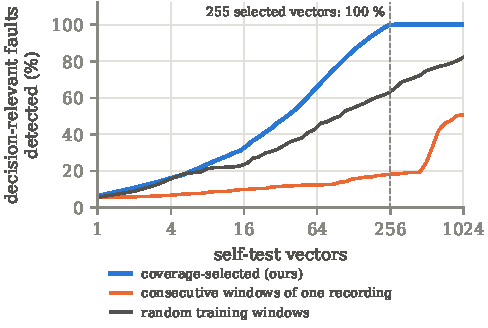
\includegraphics[width=0.72\textwidth]{figures/fault_coverage.pdf}
\caption{Decision-relevant faults detected by the first $m$ self-test vectors}\label{fig:faultcov}
\end{figure}

The natural choice of a test, 1,024 consecutive recorded windows, detects only 50.7\,\% of the faults that change a
decision; the 255 selected windows detect all of them.

\section{Board Test Campaign}\label{sec:res-board}

\begin{table}[H]
\centering\small
\caption{Board test campaign on the KV260 (kit v6 bitstream, Vivado 2026.1)}\label{tab:board}
\begin{tabularx}{\textwidth}{|P{33mm}|L|P{17mm}|}
\hline
\multicolumn{1}{|c|}{\textbf{Step}} & \multicolumn{1}{c|}{\textbf{Measured on the board}} & \multicolumn{1}{c|}{\textbf{Result}}\\
\hline
1 Identity & core version 3, 38 features, 50 LUTs; bitstream loads in 4.4\,s & PASS\\
\hline
2 Self-test & 1,024 of 1,024 vectors correct in 1,028 cycles & PASS\\
\hline
3 Latency & 3 clock cycles (30\,ns) & PASS\\
\hline
4 Replay & all 431,960 windows of 10 recordings through the registers: 0 mismatches at both operating points;
3.2\,\textmu s per window & PASS\\
\hline
5 Detection (10 recordings) & frozen point: 1 of 19 seizures, 0 false alarms in 120\,h; programmable point: 3 of 19,
25 false alarms (equal to simulation) & reported\\
\hline
6 Power & 3.069\,W idle, 3.074\,W with the classifier fed one window per clock (difference within the sensor's
noise) & reported\\
\hline
7 Front end on the Arm & 3 raw recordings: 0 feature and 0 output mismatches, 3,390--4,080 times faster than real
time & PASS\\
\hline
8 Fault injection & all 3,592 faults injected: 0 hardware/software mismatches; all 2,890 decision-relevant faults
detected; 88\,s & PASS\\
\hline
9 Whole detector in the fabric & 9,214 windows from raw samples: 0 feature and 0 output mismatches; engine busy for
exactly the simulated cycles (787,615 / 787,521 / 946,168 per second); 102--124 times faster than real time & PASS\\
\hline
\end{tabularx}
\end{table}

Step 5 covers only the 10 exported recordings of three test patients, as a check that the board reproduces the
software. The first board run found one software bug: the driver wrote ``soft reset'' and ``clear counters'' in the
same register write, and the hardware gives the reset priority, so the counters were not cleared. The driver now writes
them separately (no rebuild was needed).

\section{Analog Front-End Specification}\label{sec:res-afe}

\textbf{One impairment at a time.} Of the 40 families, 29 have a limit, 10 are tolerated even at the most severe level
tested, and one is not tolerated at any level: the ECG low-pass filter fails even at 100\,Hz. Figure~\ref{fig:toleeg}
shows the EEG curves. The detector is most sensitive to mains interference on the EEG (1\,\textmu V of 50\,Hz is
tolerated, 10\,\textmu V is not), so common-mode rejection or a notch matters more than the noise floor.

\begin{figure}[H]
\centering
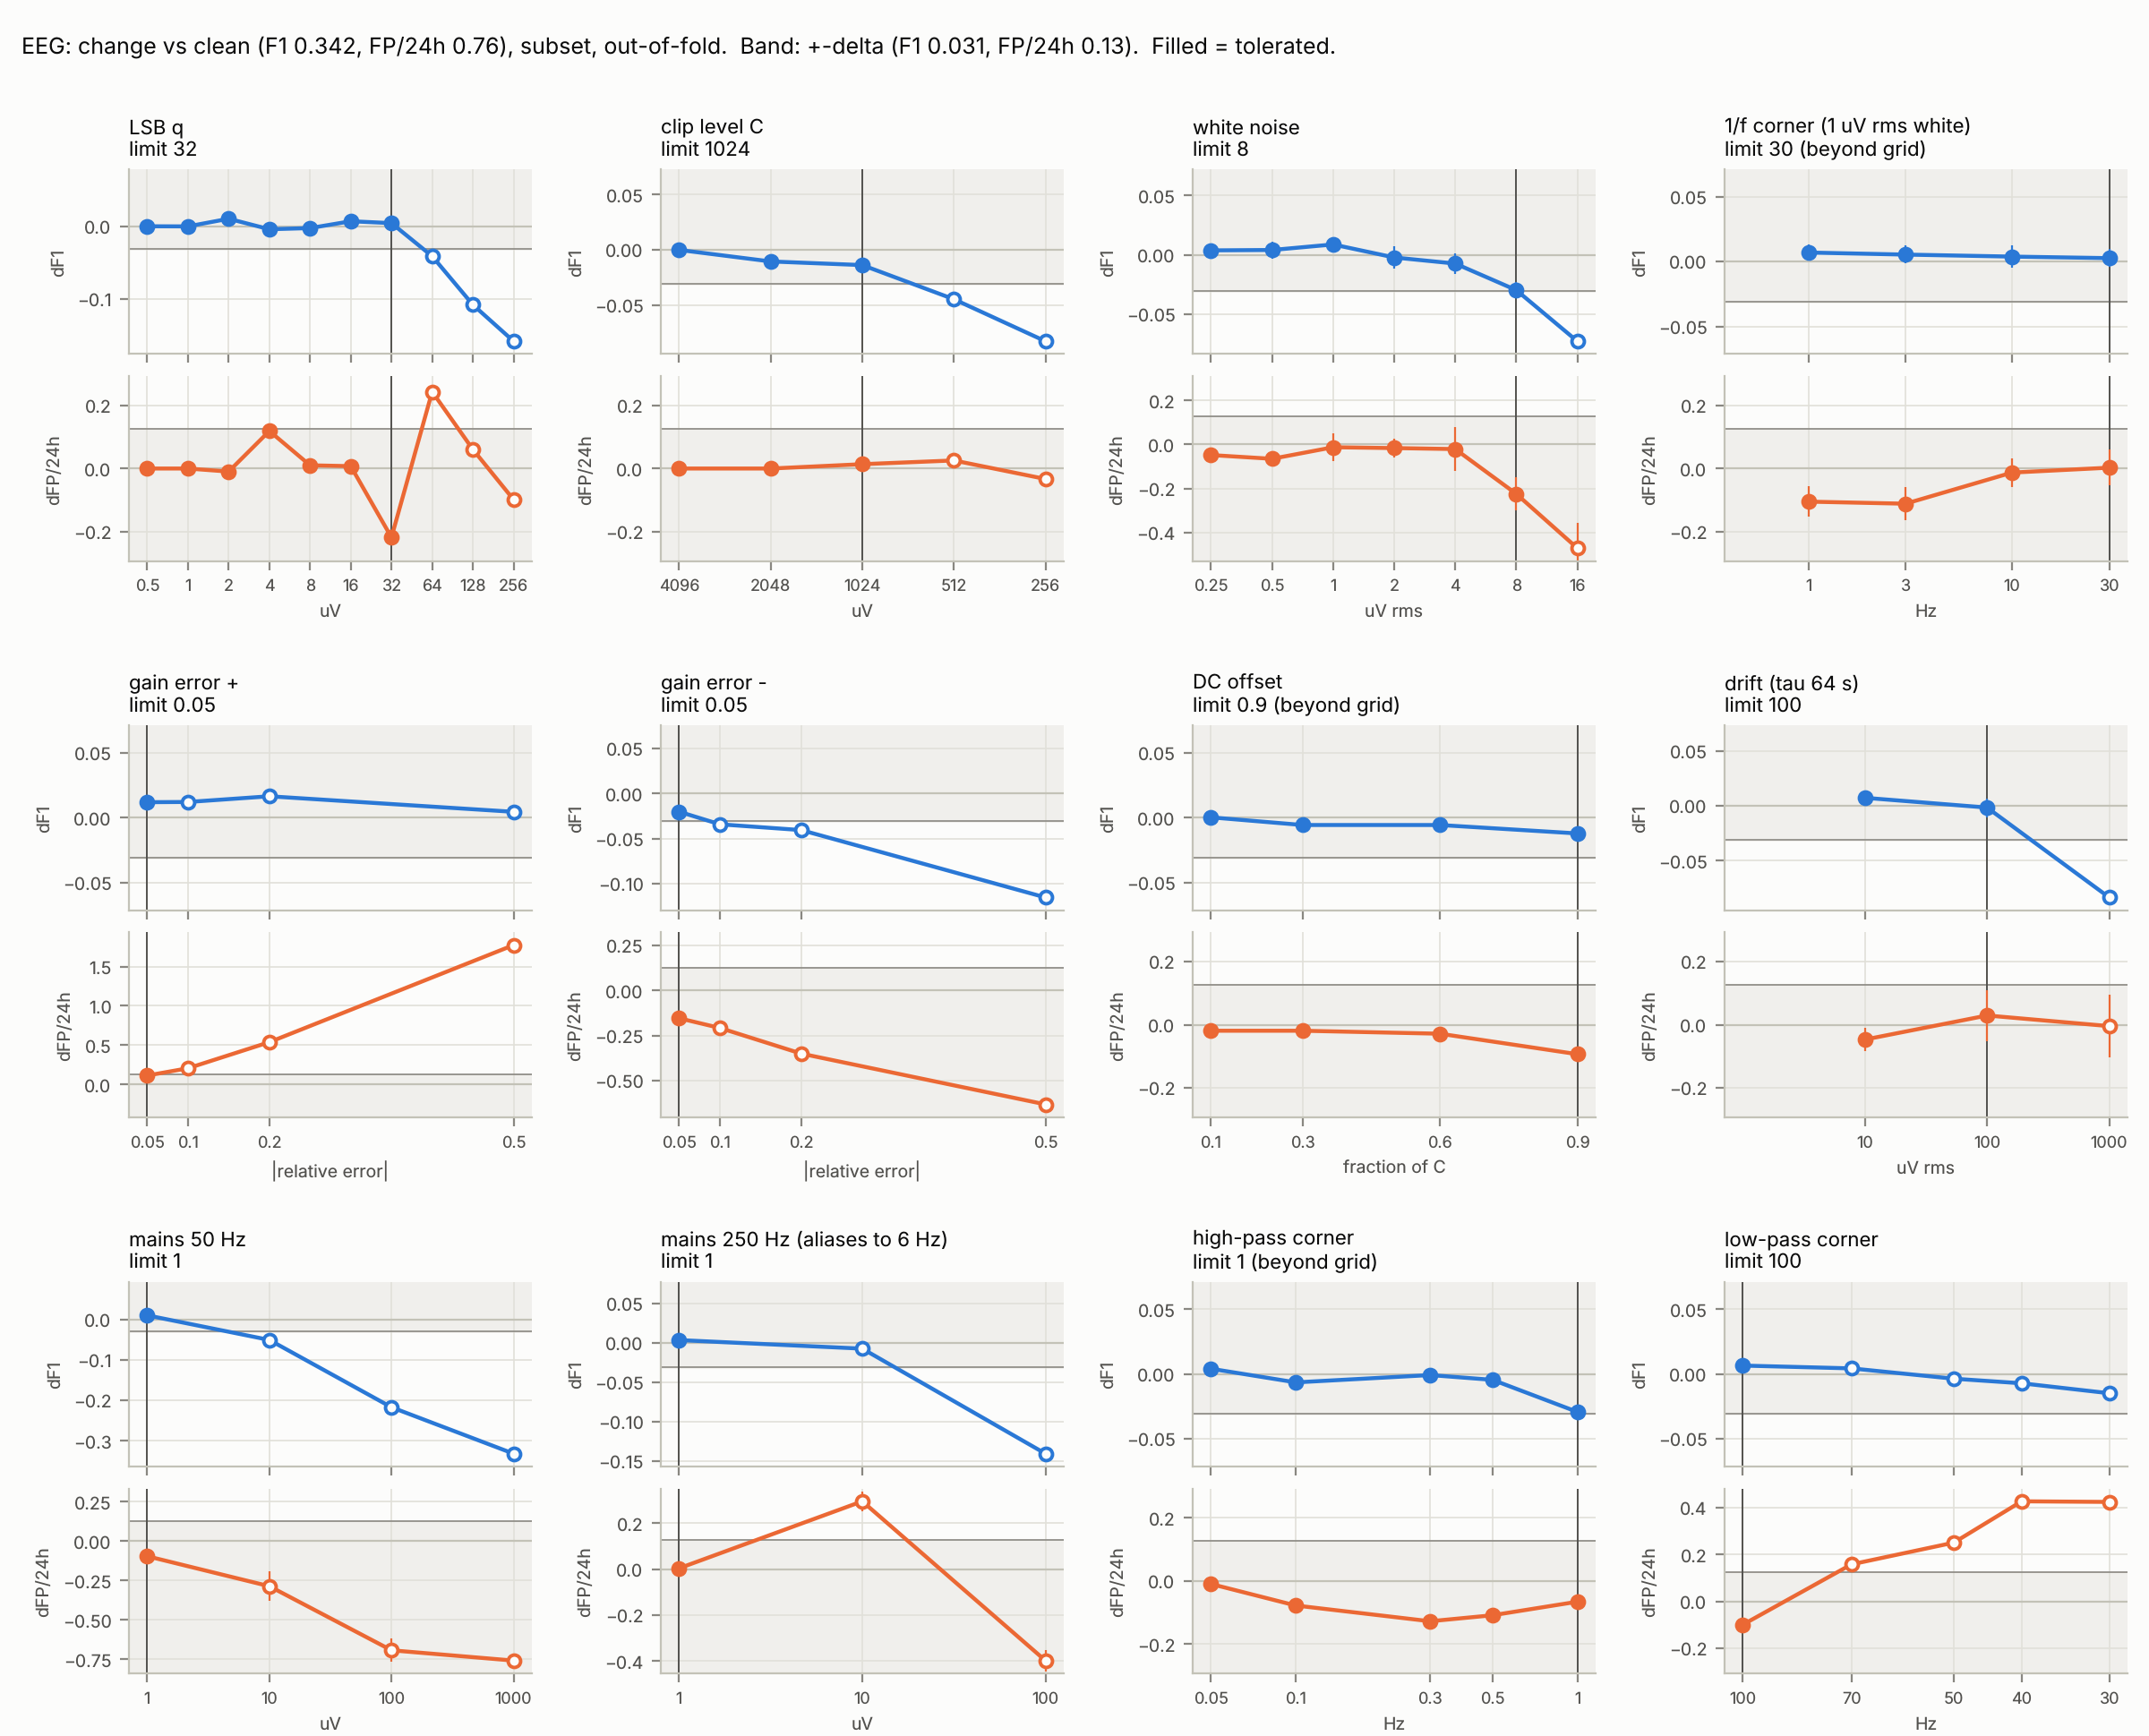
\includegraphics[width=0.95\textwidth]{figures/tolerance_eeg.png}
\caption{EEG tolerance curves on the training subset: change in event-F1 (blue) and false alarms per day (orange)
against each impairment level; filled points are tolerated}\label{fig:toleeg}
\end{figure}

\textbf{All at once.} With every family at its single-impairment limit, the F1 drop was 2.3--2.8 times the allowed
value, because each limit had used the whole error budget by itself. After 22 back-off steps the combined point passed
on the subset, and then on all 8,714.7 training hours with no further step (F1 change $-0.0022$ and $-0.0076$ for the
two signs of gain error; false alarms $+0.105$ and $+0.094$ per day; Wilcoxon $p = 0.48$ and $0.50$).

\begin{table}[H]
\centering\small
\caption{Front-end specification: limit with one impairment at a time and the combined point (all training hours)}\label{tab:afe}
\begin{tabularx}{\textwidth}{|P{20mm}|L|P{36mm}|P{36mm}|}
\hline
\multicolumn{1}{|c|}{\textbf{Signal}} & \multicolumn{1}{c|}{\textbf{Parameter}} & \multicolumn{1}{c|}{\textbf{One at a time}} & \multicolumn{1}{c|}{\textbf{Specification}}\\
\hline
EEG & input noise (0.5--100 Hz) & 4 \textmu V rms & \textbf{1 \textmu V rms}\\
\hline
EEG & ADC step / clip level & 32 \textmu V / 2048 \textmu V & \textbf{4 \textmu V / 2048 \textmu V (10 bits)}\\
\hline
EEG & 50 Hz interference & 1 \textmu V & 1 \textmu V\\
\hline
EEG & high-pass / low-pass corner & 0.5 Hz / 100 Hz & 0.1 Hz / 100 Hz\\
\hline
ECG & input noise & 8 \textmu V rms & \textbf{4 \textmu V rms}\\
\hline
ECG & ADC step / clip level & 32 \textmu V / 1024 \textmu V & \textbf{16 \textmu V / 1024 \textmu V (7 bits)}\\
\hline
ECG & low-pass corner & none tolerated & not included\\
\hline
EMG & input noise & 2 \textmu V rms & \textbf{2 \textmu V rms}\\
\hline
EMG & ADC step / clip level & $\ge$ 256 \textmu V / 1024 \textmu V & \textbf{16 \textmu V / 1024 \textmu V (7 bits)}\\
\hline
Motion & ADC step / noise & 16 LSB / 2 LSB rms & 8 LSB / 1 LSB rms\\
\hline
\end{tabularx}
\end{table}

\begin{table}[H]
\centering\small
\caption{Power of the analog front end at the specification (noise-set amplifier bound for an assumed NEF of 2, 3 and 5; ADC
power from the Murmann survey)}\label{tab:afepower}
\begin{tabular}{|l|c|c|c|c|c|}
\hline
\multicolumn{1}{|c|}{\textbf{Channels}} & \textbf{Noise density} & \textbf{NEF 2} & \textbf{NEF 3} & \textbf{NEF 5} & \textbf{ADC bits}\\
\hline
EEG (2), per channel & 100 nV/$\sqrt{\mathrm{Hz}}$ & 482 nW & 1.08 \textmu W & 3.01 \textmu W & 10\\
\hline
ECG (1) & 401 nV/$\sqrt{\mathrm{Hz}}$ & 30.1 nW & 67.8 nW & 188 nW & 7\\
\hline
EMG (1) & 201 nV/$\sqrt{\mathrm{Hz}}$ & 120 nW & 271 nW & 753 nW & 7\\
\hline
\textbf{All 4 channels} & & \textbf{1.11 \textmu W} & \textbf{2.51 \textmu W} & \textbf{6.97 \textmu W} & \\
\hline
\end{tabular}
\end{table}

The ADCs of the lowest-power real low-rate designs in the survey add about 941\,nW for all channels. The analog front end
therefore needs a few microwatts, set mainly by the EEG amplifiers: tightening the EEG noise from 4 to 1\,\textmu V rms
costs 16 times the amplifier current at the same NEF.

\textbf{FPGA impairment emulator.} The Verilog emulator matched the Python impairment model word for word in 11 test
cases of 70,000 samples each (0 mismatches; flipping one seed bit changed 65,702 of 70,000 words, which shows the
comparison works), both on its own and behind AXI4-Lite. It takes 4,713 LUTs (5,117 with AXI) in Yosys. Its run on the
board is still to be done.

\section{Live Demonstration and Doctor Alert}\label{sec:res-demo}

On the board, recorded test-patient signals stream second by second through the fabric; the alarm fires during the
seizure and the red LED and the buzzer turn on. Figure~\ref{fig:dashboard} shows the dashboard and
Figure~\ref{fig:alertpage} the doctor's page.

\begin{figure}[H]
\centering
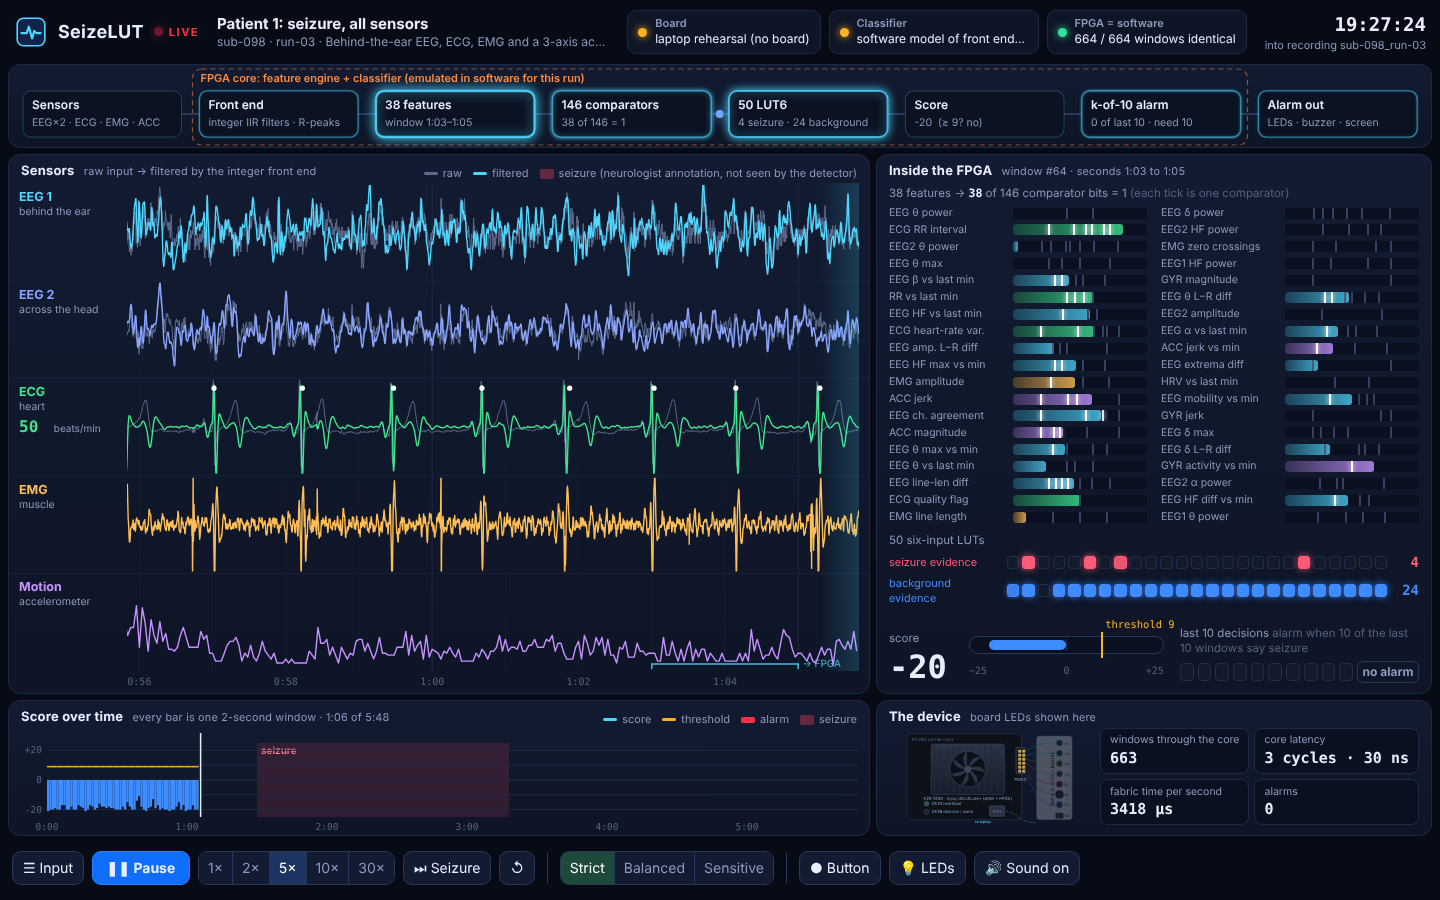
\includegraphics[width=\textwidth]{figures/dashboard_rehearsal.png}
\caption{Live dashboard: signals, features, comparator bits, LUT votes, score and alarm, with the check that the FPGA
equals the software (laptop rehearsal with the software model of the core; on the board the same page shows the
FPGA)}\label{fig:dashboard}
\end{figure}

\begin{figure}[H]
\centering
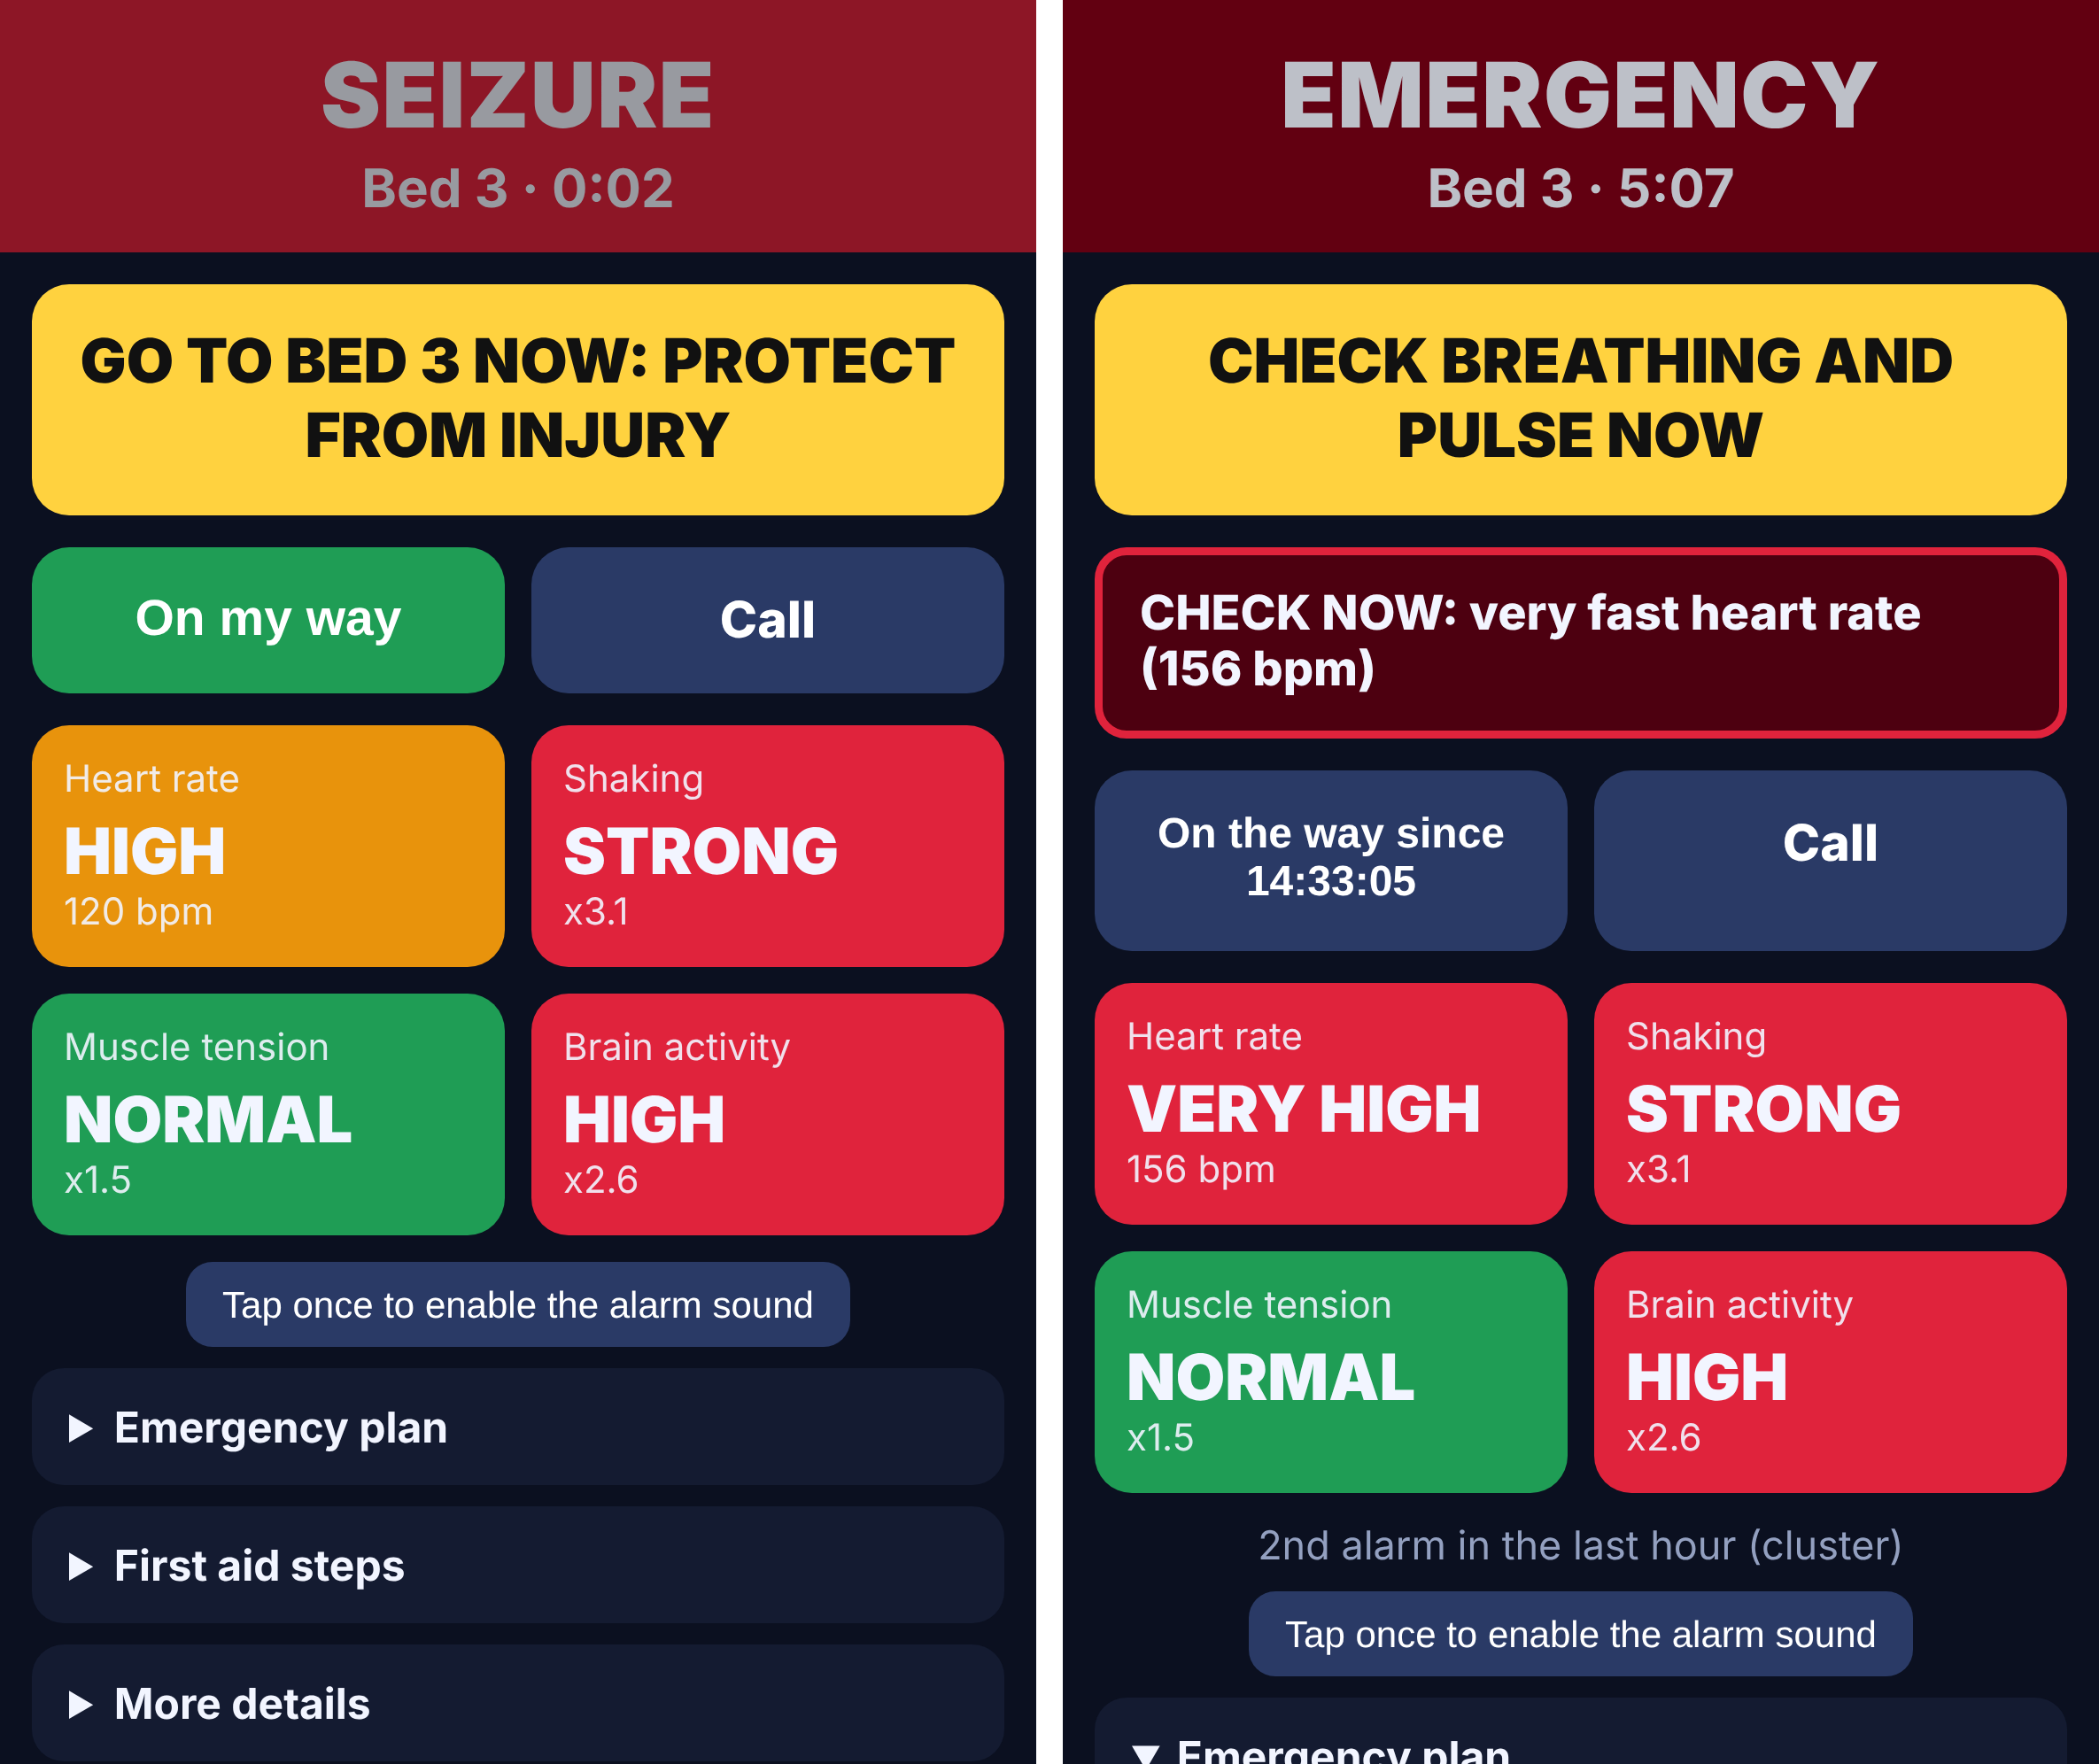
\includegraphics[width=0.85\textwidth]{figures/alert_page.png}
\caption{The doctor's page at a new seizure (left) and in an emergency after 5 minutes (right)}\label{fig:alertpage}
\end{figure}

The alert was tested on the emulated board through a virtual serial port: alarm start, updates, end after 30\,s of
quiet, escalation at 2, 5, 6 and 7 minutes (none after the alarm stops), clusters, and the acknowledgement coming back.
The ESP32 program passes a syntax check and the page was rendered at iPhone size. The test on the ESP32 itself, with a
real iPhone, is the next step.

\chapter{DISCUSSION}\label{ch:discussion}

\section{Accuracy per Lookup Table}

The final DWN is not the most accurate model: LightGBM reaches an event-F1 of 0.308 against 0.248. But LightGBM needs
about 30,800 LUTs, while the DWN needs 398 (and the whole detector 1,202). Among the models that can be built as small
multiplier-free hardware, the DWN is the most accurate, and it is above TreeLUT at a seventh of its LUTs. Distillation
from LightGBM was the most useful single change: it cut the false alarms from 2.4 to 0.9 per day on the training
patients and carried part of the teacher's accuracy into 50 truth tables.

\section{Self-Testing}

Because the classifier is a set of truth tables, every single hardware fault can be listed and its clinical effect
measured. This showed that the obvious test, replaying a block of recorded data, misses about half of the faults that
change a decision, because many truth-table entries are used only by rare inputs. Choosing test windows for coverage
closes this gap with 255 windows. The board campaign confirmed every prediction: all 3,592 injected faults behaved on
the FPGA exactly as in the software model.

\section{Challenges Faced}

\begin{xltabular}{\textwidth}{|P{17mm}|P{38mm}|L|L|}
\caption{The main problems and their solutions}\label{tab:challenges}\\
\hline
\multicolumn{1}{|c|}{\textbf{Area}} & \multicolumn{1}{c|}{\textbf{Challenge}} & \multicolumn{1}{c|}{\textbf{What happened}} & \multicolumn{1}{c|}{\textbf{Solution}}\\
\hline
\endfirsthead
\hline
\multicolumn{1}{|c|}{\textbf{Area}} & \multicolumn{1}{c|}{\textbf{Challenge}} & \multicolumn{1}{c|}{\textbf{What happened}} & \multicolumn{1}{c|}{\textbf{Solution}}\\
\hline
\endhead
\small Data & \small Files differ from the documentation & \small 256 Hz not 250 Hz; 883 not 886 seizures; no centre
or age labels & \small Full audit first; design follows the files\\ \hline
\small Data & \small 126 GB, no local disk or GPU & \small Dataset too large for the server & \small Stream, extract,
delete: only 3.5 GB of features kept\\ \hline
\small Data & \small Silent download truncation & \small 9 recordings cut short & \small Size checks; re-extracted; 3
runs repeated\\ \hline
\small Baseline & \small ChronoNet only partly reproduced & \small 74.5\,\% vs 84.2\,\% detected & \small Literal port;
gap reported as measured\\ \hline
\small Baseline & \small Released code tunes on the test patients & \small Best epoch picked on the evaluation patients &
\small Clean run with no test information as our reference\\ \hline
\small Hardware & \small Rounding noise in integer filters & \small Error 140 LSB, larger than the signal (61 LSB) &
\small Error feedback: 0.7 LSB\\ \hline
\small Hardware & \small Heart rate needs a division & \small $60/\mathrm{RR}$ & \small $\log_2(\mathrm{RR})$: no division
or multiplication\\ \hline
\small Compute & \small 6 GB laptop GPU; CUDA-only library & \small DWN could not run on the CPU server & \small PyTorch
re-implementation, unit-tested against the kernel\\ \hline
\small ML & \small Seizures are 0.123\,\% of the time & \small Accuracy is meaningless & \small Event scoring per
patient; balanced sampling; false-alarm budget\\ \hline
\small ML & \small Weak early results & \small First network: event-F1 0.148, 7.0 false alarms per day & \small N7 showed
heart rate was ignored; new feature selection: 0.208, 2.3 per day\\ \hline
\small FPGA & \small Front end needs many multipliers & \small Dozens of filters per window & \small Microcoded shift-add
engine: 804 LUTs, no DSP\\ \hline
\small FPGA & \small Engine and bus raced each other & \small For one clock cycle the core reported idle before the
feature transfer, and writes were lost & \small Found by the end-to-end testbench before the build; idle condition
fixed\\ \hline
\small Board & \small Counters not cleared on the board & \small Reset and clear in one write & \small Two separate
writes\\ \hline
\small Demo & \small LED always on, buzzer silent & \small Wires on the wrong end of the PMOD connector; buzzer (+) not
on 3.3\,V & \small Pin test script; wiring table\\ \hline
\small Alert & \small Too much information for a doctor in a hurry & \small Long text with numbers & \small One
instruction, four colour tiles, three-line notification\\ \hline
\small Alert & \small False ``check breathing'' during shaking & \small Shaking spoils the ECG & \small ECG flag only
without shaking\\ \hline
\end{xltabular}

\section{Limitations}

\begin{itemize}
\item \textbf{Focal seizures:} at the default operating point the detector finds about one seizure in four, and focal
  seizures are mostly missed, as in the clinical literature \cite{beniczky2021guideline}.
\item \textbf{Retrospective data:} all results come from recordings of one dataset; no patient wore our hardware.
\item \textbf{Two-stage detector:} the 73.3\,\% result needs a 96\,s decision delay and about 11 false alarms per
  hour, so it suits seizure logging rather than instant alarms.
\item \textbf{Self-adaptation:} label-free per-patient adaptation (N3) raised the false alarms from 6.8 to 10--40 per
  day on the training patients and was not adopted.
\item \textbf{Doctor alert:} tested in emulation only; the pattern hint matches the doctors' label in 64\,\% of
  training seizures and is not a diagnosis.
\end{itemize}

\chapter{CONCLUSION AND FUTURE SCOPE}\label{ch:concl}

\section{Conclusion}

SeizeLUT demonstrates a complete, multiplier-free seizure detector on FPGA hardware. A 50-LUT weightless network on
integer features from behind-the-ear EEG, ECG, EMG and motion reaches an event-F1 of 0.248 with 0.8 false alarms per
day on 29 held-out patients, above TreeLUT, the logic-gate network, the INT8 network and ChronoNet, in 398 LUTs; with
its microcoded front end in the fabric the whole detector needs 1,202 LUTs and no multiplier. At equal false alarms it
detects more seizures than ChronoNet (43.2\,\% against 34.8\,\%), and with post-ictal verification it detects more
than the dataset paper's SVM at its false-alarm rate (73.3\,\% against 71.1\,\%). All 3,592 single faults of the
classifier were analysed, and 255 selected test vectors detect every fault that changes a decision, in a 10.3\,\textmu s
on-chip self-test. On the AMD Kria KV260 all nine board tests pass, the board equals the software on every window and
every injected fault. Driving the detector with impaired signals gave a specification for its analog front end (EEG noise
1\,\textmu V rms, 10-bit EEG and 7-bit ECG and EMG converters, a few microwatts in total). A live demonstration drives an alarm LED and a buzzer while an ESP32 tells the doctor what to
do.

\section{Future Scope}

\begin{itemize}
\item Test the doctor alert on the ESP32 with a real phone and measure the time from alarm to notification.
\item Learn each patient from doctor feedback (``real seizure'' or ``false alarm'') and retrain the truth tables, with
  new self-test vectors for every update.
\item Detect more focal seizures, the main clinical gap.
\item Record volunteers wearing the sensors with a battery-powered low-power FPGA, and run the self-test periodically
  in the field.
\item Design the front end to the derived specification (SKY130 comparator, FPGA delta-sigma ADC) and run the
  impairment emulator on the board.
\item Submit the work as a paper (IEEE EMBC 2027, full paper deadline 24 January 2027).
\end{itemize}


% ================================================================ references and appendices
\cleardoublepage
\phantomsection
\addcontentsline{toc}{chapter}{References}
{\small\setstretch{1.1}
\bibliographystyle{IEEEtran}
\bibliography{refs}}

\appendix
% appendices: "APPENDIX A: TITLE" headings, tables numbered A.1, B.1
\cleardoublepage
\refstepcounter{chapter}\label{app:build}
\chapter*{APPENDIX A: BUILD INSTRUCTIONS AND SOURCE FILES}
\addcontentsline{toc}{chapter}{APPENDIX A: BUILD INSTRUCTIONS AND SOURCE FILES}

The bitstream is built with Vivado 2026.1 by \texttt{hw/kv260/vivado/build\_kv260.tcl}, which also writes the
utilisation, timing and power reports. On the board (Ubuntu 22.04 with Kria-PYNQ), the kit folder is copied to the
home directory and the test campaign is run with \texttt{bash run\_board\_tests.sh} (\texttt{--quick} for a one-minute
check). The live demonstration with the LED and buzzer is started with \texttt{bash demo2\_components.sh --autoplay
--speed 4}, and the doctor alert by adding \texttt{--bed "Bed 1"} once the ESP32 is connected. The ESP32 program is
uploaded from the Arduino IDE (board: ESP32 Dev Module) after the Wi-Fi name, password and ntfy topic are set at the top
of the sketch.

\begin{table}[H]
\centering\small
\caption{Source files of the project}\label{tab:sourcefiles}
\begin{tabularx}{\textwidth}{|P{62mm}|L|}
\hline
\multicolumn{1}{|c|}{\textbf{File}} & \multicolumn{1}{c|}{\textbf{Contents}}\\
\hline
\texttt{src/features/golden.py} & Integer front end (golden model)\\
\hline
\texttt{src/hw/fe\_engine.py}, \texttt{hw/kv260/rtl/fe\_engine.v} & Feature engine: program generator and RTL\\
\hline
\texttt{src/hw/kv260.py} & Generator of the KV260 core (classifier, self-test, fault injection, AXI)\\
\hline
\texttt{export/n4\_distill\_s0/} & Final model: thresholds, input mapping, 50 truth tables, score head, test vectors\\
\hline
\texttt{hw/kv260/sim/} & Testbenches and simulation scripts\\
\hline
\texttt{hw/kv260/vivado/build\_kv260.tcl} & Vivado build script\\
\hline
\texttt{hw/kv260/board/} & Driver, test campaign (steps 1--9), fault campaign, C front end\\
\hline
\texttt{hw/kv260/demo/} & Live dashboard, demo scripts, doctor-alert link\\
\hline
\texttt{hw/kv260/esp32/seizelut\_alert/} & ESP32 alert program\\
\hline
\texttt{results/decisions.md} & Every design decision with its evidence\\
\hline
\end{tabularx}
\end{table}

\cleardoublepage
\refstepcounter{chapter}\label{app:results}
\setcounter{table}{0}
\chapter*{APPENDIX B: ALL MODELS ON THE 29 TEST PATIENTS}
\addcontentsline{toc}{chapter}{APPENDIX B: ALL MODELS ON THE 29 TEST PATIENTS}

\begin{table}[H]
\centering\footnotesize
\caption{Final evaluation of every model on the 29 test patients (5 seeds; SzCORE event metrics at the best-F1
operating point; Paper: the base paper's sensitivity and false alarms per hour; $p$: paired Wilcoxon on per-patient
event-F1 against LightGBM)}\label{tab:test-full}
\setlength{\tabcolsep}{2pt}
\begin{tabular}{|l|c|c|c|c|c|c|c|c|}
\hline
\multicolumn{1}{|c|}{\textbf{Model}} & \textbf{AUROC} & \textbf{F1} & \textbf{Sens} & \textbf{Prec} & \textbf{FA/24\,h} &
\textbf{Paper} & \textbf{Cost} & \textbf{$p$}\\
\hline
\textbf{DWN + distillation (final)} & 0.883 & \textbf{0.248} & 0.303 & 0.291 & 0.8 & 25.5\,\% / 0.02 & 895 LUTs & 0.039\\
\hline
DWN + modality dropout & 0.866 & 0.242 & 0.272 & 0.282 & 0.4 & 21.7\,\% / 0.01 & 951 LUTs & 0.035\\
\hline
DWN base & 0.875 & 0.172 & 0.340 & 0.156 & 2.7 & 29.2\,\% / 0.12 & 980 LUTs & 0.004\\
\hline
LightGBM & 0.877 & 0.308 & 0.331 & 0.396 & 0.6 & 26.8\,\% / 0.01 & 30,750 LUTs & --\\
\hline
XGBoost & 0.872 & 0.294 & 0.301 & 0.387 & 0.4 & 25.1\,\% / 0.01 & 48,295 LUTs & 0.29\\
\hline
CatBoost & 0.874 & 0.254 & 0.330 & 0.281 & 1.2 & 25.8\,\% / 0.04 & 27,720 LUTs & 0.026\\
\hline
Random forest & 0.858 & 0.246 & 0.245 & 0.305 & 0.2 & 22.4\,\% / 0.00 & 346,576 LUTs & 0.35\\
\hline
TreeLUT (5-bit leaves) & 0.858 & 0.233 & 0.292 & 0.296 & 1.0 & 25.1\,\% / 0.04 & 6,330 LUTs & 0.005\\
\hline
Logic-gate network & 0.865 & 0.191 & 0.291 & 0.186 & 1.4 & 23.1\,\% / 0.06 & 7,452 LUTs & 0.008\\
\hline
INT8 MLP & 0.788 & 0.155 & 0.249 & 0.163 & 1.7 & 21.8\,\% / 0.10 & 9,600 mult. & 0.005\\
\hline
Logistic regression & 0.814 & 0.123 & 0.255 & 0.096 & 5.1 & 23.0\,\% / 0.27 & 117 mult. & 0.0008\\
\hline
ChronoNet (clean, 1 seed) & -- & 0.027 & 0.790 & 0.015 & 106.3 & 67.1\,\% / 11.9 & CNN + GRU & --\\
\hline
\end{tabular}
\end{table}


\end{document}
